\batchmode
\documentclass{report}
\RequirePackage{ifthen}


\usepackage{amssymb}
\usepackage[dvips]{graphicx}
\usepackage{verbatim}
\usepackage{html}


\usepackage{amsmath}
\usepackage{latexsym,amssymb}
\usepackage[mathscr]{eucal}
\usepackage{amsthm,amsxtra,amscd,upref}
\usepackage{layout,bm,dcolumn}
\usepackage{graphicx,color}
\usepackage{calc}


\usepackage{framed}

%
\providecommand{\DST}[1]{{\ensuremath{\displaystyle{#1}}}}%
\providecommand{\DSF}[2]{{\ensuremath{\displaystyle{\frac{{\ensuremath{\displaystyle{#1}}}}{{\ensuremath{\displaystyle{#2}}}}}}}} 

%
\providecommand{\vk}[1]{{\ensuremath{\underline{\bm{#1}}}}}%
\providecommand{\mx}[1]{{\ensuremath{\bm{\mathsf{#1}}}}}%
\providecommand{\lrb}[1]{{\ensuremath{\left({#1}\right)}}}%
\providecommand{\lrs}[1]{{\ensuremath{\left[{#1}\right]}}}%
\providecommand{\lrc}[1]{{\ensuremath{\left\{{#1}\right\}}}}%
\providecommand{\lrv}[1]{{\ensuremath{\left|{#1}\right|}}} 

%
\providecommand{\hell}{{\ensuremath{\hat{\jmath}}}}%
\providecommand{\zell}{{\ensuremath{\mathfrak{z}}}}%
\providecommand{\vM}{{\ensuremath{{\ensuremath{\underline{\bm{M}}}}}}}%
\providecommand{\vr}{{\ensuremath{{\ensuremath{\underline{\bm{r}}}}}}}%
\providecommand{\vq}{{\ensuremath{{\ensuremath{\underline{\bm{q}}}}}}}%
\providecommand{\vh}{{\ensuremath{{\ensuremath{\underline{\bm{h}}}}}}}%
\providecommand{\vkx}{{\ensuremath{{\ensuremath{\underline{\bm{x}}}}}}}%
\providecommand{\vkxt}{{\ensuremath{{\ensuremath{\underline{\bm{x}}}}^t}}}%
\providecommand{\vky}{{\ensuremath{{\ensuremath{\underline{\bm{y}}}}}}}%
\providecommand{\vkyt}{{\ensuremath{{\ensuremath{\underline{\bm{y}}}}^t}}} 

%
\providecommand{\vri}[1]{{\ensuremath{{\ensuremath{\underline{\bm{r}}}}_{#1}}}}%
\providecommand{\vrr}{{\ensuremath{{\ensuremath{\underline{\bm{r}}}}}}}%
\providecommand{\vqi}[1]{{\ensuremath{{\ensuremath{\underline{\bm{q}}}}_{#1}}}}%
\providecommand{\vqr}{{\ensuremath{{\ensuremath{\underline{\bm{q}}}}}}}%
\providecommand{\vhi}[1]{{\ensuremath{{\ensuremath{\underline{\bm{h}}}}_{#1}}}}%
\providecommand{\vhr}{{\ensuremath{{\ensuremath{\underline{\bm{h}}}}}}}%
\providecommand{\IMA}{{\ensuremath{\mathrm{i}}}}%
\providecommand{\EE}{{\ensuremath{\mathrm{e}}}}%
\providecommand{\half}{{\ensuremath{\frac{1}{2}}}} 

%
\providecommand{\deltax}{{\ensuremath{\rho\cos(\beta)}}}%
\providecommand{\deltay}{{\ensuremath{\rho\sin(\beta)}}}%
\providecommand{\deltaz}{{\ensuremath{\delta_{z}}}}%
\providecommand{\deltazs}{{\ensuremath{\widehat{{\ensuremath{\delta_{z}}}}}}}%
\providecommand{\DD}[1]{{\ensuremath{\mathrm{d}{#1}\, }}}%
\providecommand{\DDD}[2]{{\ensuremath{\mathrm{d}^{#1}{#2}\, }}} 

%
\providecommand{\haf}{{\ensuremath{\scriptstyle{\frac{1}{2}}}}}%
\providecommand{\unt}{{\ensuremath{\scriptstyle{\frac{1}{3}}}}}%
\providecommand{\dut}{{\ensuremath{\scriptstyle{\frac{2}{3}}}}}%
\providecommand{\xref}[1]{(\ref{#1})}%
\providecommand{\eref}[1]{Eq.~(\ref{#1})}%
\providecommand{\Beref}[1]{{\textcolor[rgb]{0,0,1}{Eq.~(\ref{#1})}}}%
\providecommand{\eeref}[2]{Eqs.~(\ref{#1},\ref{#2})}%
\providecommand{\eeeref}[3]{Eqs.~(\ref{#1},\ref{#2},\ref{#3})}%
\providecommand{\aref}[1]{Appendix~\ref{#1}}%
\providecommand{\sref}[1]{Sec.~\ref{#1}}%
\providecommand{\cref}[1]{Chap.~\ref{#1}}%
\providecommand{\tref}[1]{Tab.~\ref{#1}}%
\providecommand{\fref}[1]{Fig.~\ref{#1}}%
\providecommand{\Rref}[1]{Ref.~\cite{#1}}%
\providecommand{\degC}{{\ensuremath{{}^{\mathrm{o}}}}} 

%
\providecommand{\TT}{{\ensuremath{{2\theta}}}}%
\providecommand{\TTz}{{\ensuremath{{{{\ensuremath{{2\theta}}}}_{0}}}}}%
\providecommand{\TTe}{{\ensuremath{{{{\ensuremath{{2\theta}}}}_{e}}}}}%
\providecommand{\TTB}{{\ensuremath{{{{\ensuremath{{2\theta}}}}_{B}}}}} 





\pagecolor[gray]{.7}

\usepackage[]{inputenc}



\makeatletter

\makeatletter
\count@=\the\catcode`\_ \catcode`\_=8 
\newenvironment{tex2html_wrap}{}{}%
\catcode`\<=12\catcode`\_=\count@
\newcommand{\providedcommand}[1]{\expandafter\providecommand\csname #1\endcsname}%
\newcommand{\renewedcommand}[1]{\expandafter\providecommand\csname #1\endcsname{}%
  \expandafter\renewcommand\csname #1\endcsname}%
\newcommand{\newedenvironment}[1]{\newenvironment{#1}{}{}\renewenvironment{#1}}%
\let\newedcommand\renewedcommand
\let\renewedenvironment\newedenvironment
\makeatother
\let\mathon=$
\let\mathoff=$
\ifx\AtBeginDocument\undefined \newcommand{\AtBeginDocument}[1]{}\fi
\newbox\sizebox
\setlength{\hoffset}{0pt}\setlength{\voffset}{0pt}
\addtolength{\textheight}{\footskip}\setlength{\footskip}{0pt}
\addtolength{\textheight}{\topmargin}\setlength{\topmargin}{0pt}
\addtolength{\textheight}{\headheight}\setlength{\headheight}{0pt}
\addtolength{\textheight}{\headsep}\setlength{\headsep}{0pt}
\setlength{\textwidth}{349pt}
\newwrite\lthtmlwrite
\makeatletter
\let\realnormalsize=\normalsize
\global\topskip=2sp
\def\preveqno{}\let\real@float=\@float \let\realend@float=\end@float
\def\@float{\let\@savefreelist\@freelist\real@float}
\def\liih@math{\ifmmode$\else\bad@math\fi}
\def\end@float{\realend@float\global\let\@freelist\@savefreelist}
\let\real@dbflt=\@dbflt \let\end@dblfloat=\end@float
\let\@largefloatcheck=\relax
\let\if@boxedmulticols=\iftrue
\def\@dbflt{\let\@savefreelist\@freelist\real@dbflt}
\def\adjustnormalsize{\def\normalsize{\mathsurround=0pt \realnormalsize
 \parindent=0pt\abovedisplayskip=0pt\belowdisplayskip=0pt}%
 \def\phantompar{\csname par\endcsname}\normalsize}%
\def\lthtmltypeout#1{{\let\protect\string \immediate\write\lthtmlwrite{#1}}}%
\newcommand\lthtmlhboxmathA{\adjustnormalsize\setbox\sizebox=\hbox\bgroup\kern.05em }%
\newcommand\lthtmlhboxmathB{\adjustnormalsize\setbox\sizebox=\hbox to\hsize\bgroup\hfill }%
\newcommand\lthtmlvboxmathA{\adjustnormalsize\setbox\sizebox=\vbox\bgroup %
 \let\ifinner=\iffalse \let\)\liih@math }%
\newcommand\lthtmlboxmathZ{\@next\next\@currlist{}{\def\next{\voidb@x}}%
 \expandafter\box\next\egroup}%
\newcommand\lthtmlmathtype[1]{\gdef\lthtmlmathenv{#1}}%
\newcommand\lthtmllogmath{\dimen0\ht\sizebox \advance\dimen0\dp\sizebox
  \ifdim\dimen0>.95\vsize
   \lthtmltypeout{%
*** image for \lthtmlmathenv\space is too tall at \the\dimen0, reducing to .95 vsize ***}%
   \ht\sizebox.95\vsize \dp\sizebox\z@ \fi
  \lthtmltypeout{l2hSize %
:\lthtmlmathenv:\the\ht\sizebox::\the\dp\sizebox::\the\wd\sizebox.\preveqno}}%
\newcommand\lthtmlfigureA[1]{\let\@savefreelist\@freelist
       \lthtmlmathtype{#1}\lthtmlvboxmathA}%
\newcommand\lthtmlpictureA{\bgroup\catcode`\_=8 \lthtmlpictureB}%
\newcommand\lthtmlpictureB[1]{\lthtmlmathtype{#1}\egroup
       \let\@savefreelist\@freelist \lthtmlhboxmathB}%
\newcommand\lthtmlpictureZ[1]{\hfill\lthtmlfigureZ}%
\newcommand\lthtmlfigureZ{\lthtmlboxmathZ\lthtmllogmath\copy\sizebox
       \global\let\@freelist\@savefreelist}%
\newcommand\lthtmldisplayA{\bgroup\catcode`\_=8 \lthtmldisplayAi}%
\newcommand\lthtmldisplayAi[1]{\lthtmlmathtype{#1}\egroup\lthtmlvboxmathA}%
\newcommand\lthtmldisplayB[1]{\edef\preveqno{(\theequation)}%
  \lthtmldisplayA{#1}\let\@eqnnum\relax}%
\newcommand\lthtmldisplayZ{\lthtmlboxmathZ\lthtmllogmath\lthtmlsetmath}%
\newcommand\lthtmlinlinemathA{\bgroup\catcode`\_=8 \lthtmlinlinemathB}
\newcommand\lthtmlinlinemathB[1]{\lthtmlmathtype{#1}\egroup\lthtmlhboxmathA
  \vrule height1.5ex width0pt }%
\newcommand\lthtmlinlineA{\bgroup\catcode`\_=8 \lthtmlinlineB}%
\newcommand\lthtmlinlineB[1]{\lthtmlmathtype{#1}\egroup\lthtmlhboxmathA}%
\newcommand\lthtmlinlineZ{\egroup\expandafter\ifdim\dp\sizebox>0pt %
  \expandafter\centerinlinemath\fi\lthtmllogmath\lthtmlsetinline}
\newcommand\lthtmlinlinemathZ{\egroup\expandafter\ifdim\dp\sizebox>0pt %
  \expandafter\centerinlinemath\fi\lthtmllogmath\lthtmlsetmath}
\newcommand\lthtmlindisplaymathZ{\egroup %
  \centerinlinemath\lthtmllogmath\lthtmlsetmath}
\def\lthtmlsetinline{\hbox{\vrule width.1em \vtop{\vbox{%
  \kern.1em\copy\sizebox}\ifdim\dp\sizebox>0pt\kern.1em\else\kern.3pt\fi
  \ifdim\hsize>\wd\sizebox \hrule depth1pt\fi}}}
\def\lthtmlsetmath{\hbox{\vrule width.1em\kern-.05em\vtop{\vbox{%
  \kern.1em\kern0.8 pt\hbox{\hglue.17em\copy\sizebox\hglue0.8 pt}}\kern.3pt%
  \ifdim\dp\sizebox>0pt\kern.1em\fi \kern0.8 pt%
  \ifdim\hsize>\wd\sizebox \hrule depth1pt\fi}}}
\def\centerinlinemath{%
  \dimen1=\ifdim\ht\sizebox<\dp\sizebox \dp\sizebox\else\ht\sizebox\fi
  \advance\dimen1by.5pt \vrule width0pt height\dimen1 depth\dimen1 
 \dp\sizebox=\dimen1\ht\sizebox=\dimen1\relax}

\def\lthtmlcheckvsize{\ifdim\ht\sizebox<\vsize 
  \ifdim\wd\sizebox<\hsize\expandafter\hfill\fi \expandafter\vfill
  \else\expandafter\vss\fi}%
\providecommand{\selectlanguage}[1]{}%
\makeatletter \tracingstats = 1 
\providecommand{\Beta}{\textrm{B}}
\providecommand{\Mu}{\textrm{M}}
\providecommand{\Kappa}{\textrm{K}}
\providecommand{\Rho}{\textrm{R}}
\providecommand{\Epsilon}{\textrm{E}}
\providecommand{\Chi}{\textrm{X}}
\providecommand{\Iota}{\textrm{J}}
\providecommand{\omicron}{\textrm{o}}
\providecommand{\Zeta}{\textrm{Z}}
\providecommand{\Eta}{\textrm{H}}
\providecommand{\Omicron}{\textrm{O}}
\providecommand{\Nu}{\textrm{N}}
\providecommand{\Tau}{\textrm{T}}
\providecommand{\Alpha}{\textrm{A}}


\begin{document}
\pagestyle{empty}\thispagestyle{empty}\lthtmltypeout{}%
\lthtmltypeout{latex2htmlLength hsize=\the\hsize}\lthtmltypeout{}%
\lthtmltypeout{latex2htmlLength vsize=\the\vsize}\lthtmltypeout{}%
\lthtmltypeout{latex2htmlLength hoffset=\the\hoffset}\lthtmltypeout{}%
\lthtmltypeout{latex2htmlLength voffset=\the\voffset}\lthtmltypeout{}%
\lthtmltypeout{latex2htmlLength topmargin=\the\topmargin}\lthtmltypeout{}%
\lthtmltypeout{latex2htmlLength topskip=\the\topskip}\lthtmltypeout{}%
\lthtmltypeout{latex2htmlLength headheight=\the\headheight}\lthtmltypeout{}%
\lthtmltypeout{latex2htmlLength headsep=\the\headsep}\lthtmltypeout{}%
\lthtmltypeout{latex2htmlLength parskip=\the\parskip}\lthtmltypeout{}%
\lthtmltypeout{latex2htmlLength oddsidemargin=\the\oddsidemargin}\lthtmltypeout{}%
\makeatletter
\if@twoside\lthtmltypeout{latex2htmlLength evensidemargin=\the\evensidemargin}%
\else\lthtmltypeout{latex2htmlLength evensidemargin=\the\oddsidemargin}\fi%
\lthtmltypeout{}%
\makeatother
\setcounter{page}{1}
\onecolumn

% !!! IMAGES START HERE !!!

{\newpage\clearpage
\lthtmlinlinemathA{tex2html_wrap_inline7663}%
$ \chi ^2$%
\lthtmlinlinemathZ
\lthtmlcheckvsize\clearpage}

\stepcounter{chapter}
\stepcounter{section}
\stepcounter{section}
{\newpage\clearpage
\lthtmlpictureA{tex2html_wrap7743}%
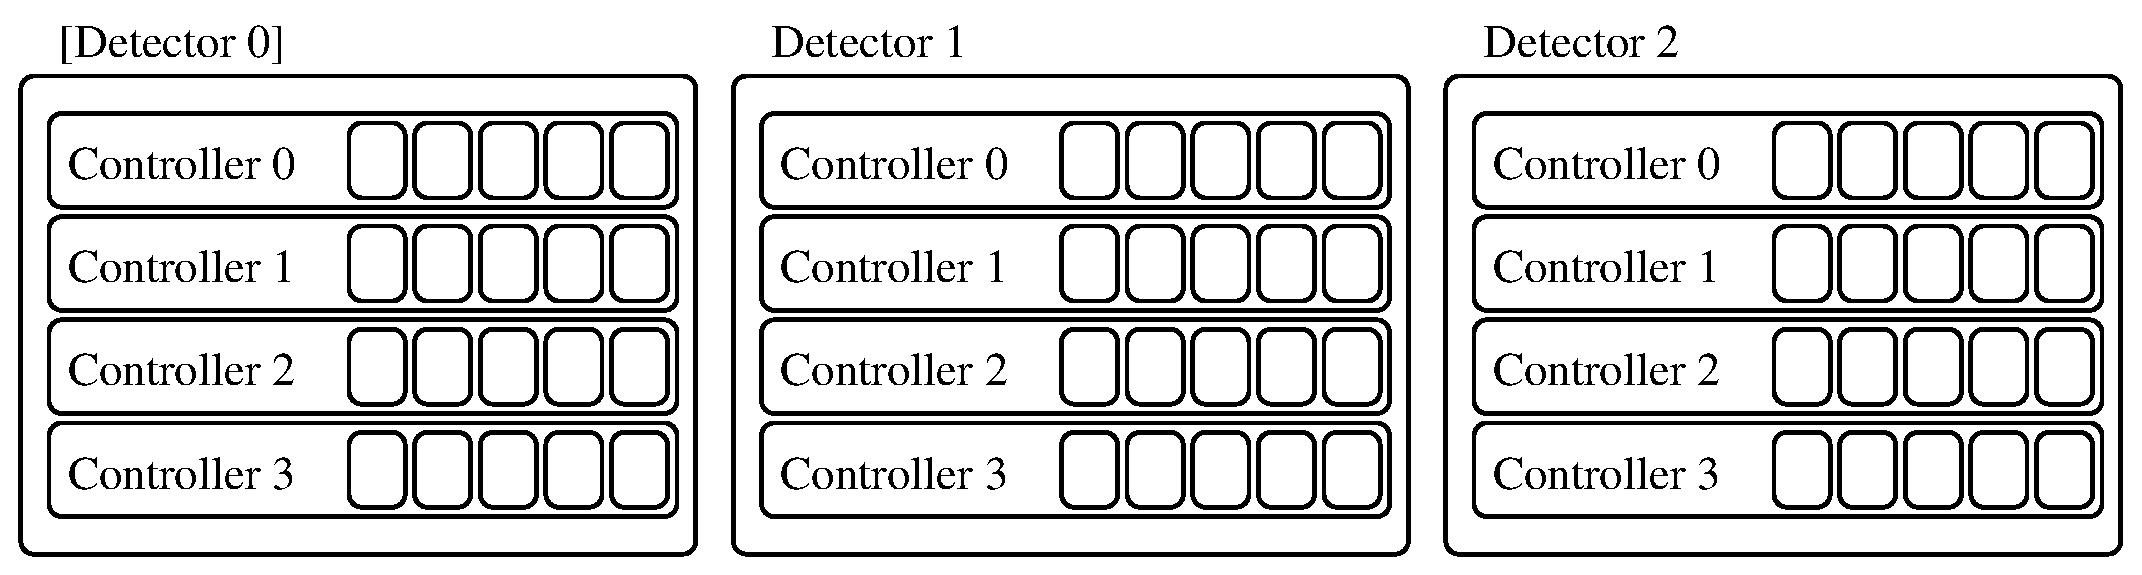
\includegraphics[width=\textwidth]{multi_detector}%
\lthtmlpictureZ
\lthtmlcheckvsize\clearpage}

\stepcounter{subsection}
\stepcounter{section}
{\newpage\clearpage
\lthtmlpictureA{tex2html_wrap7749}%
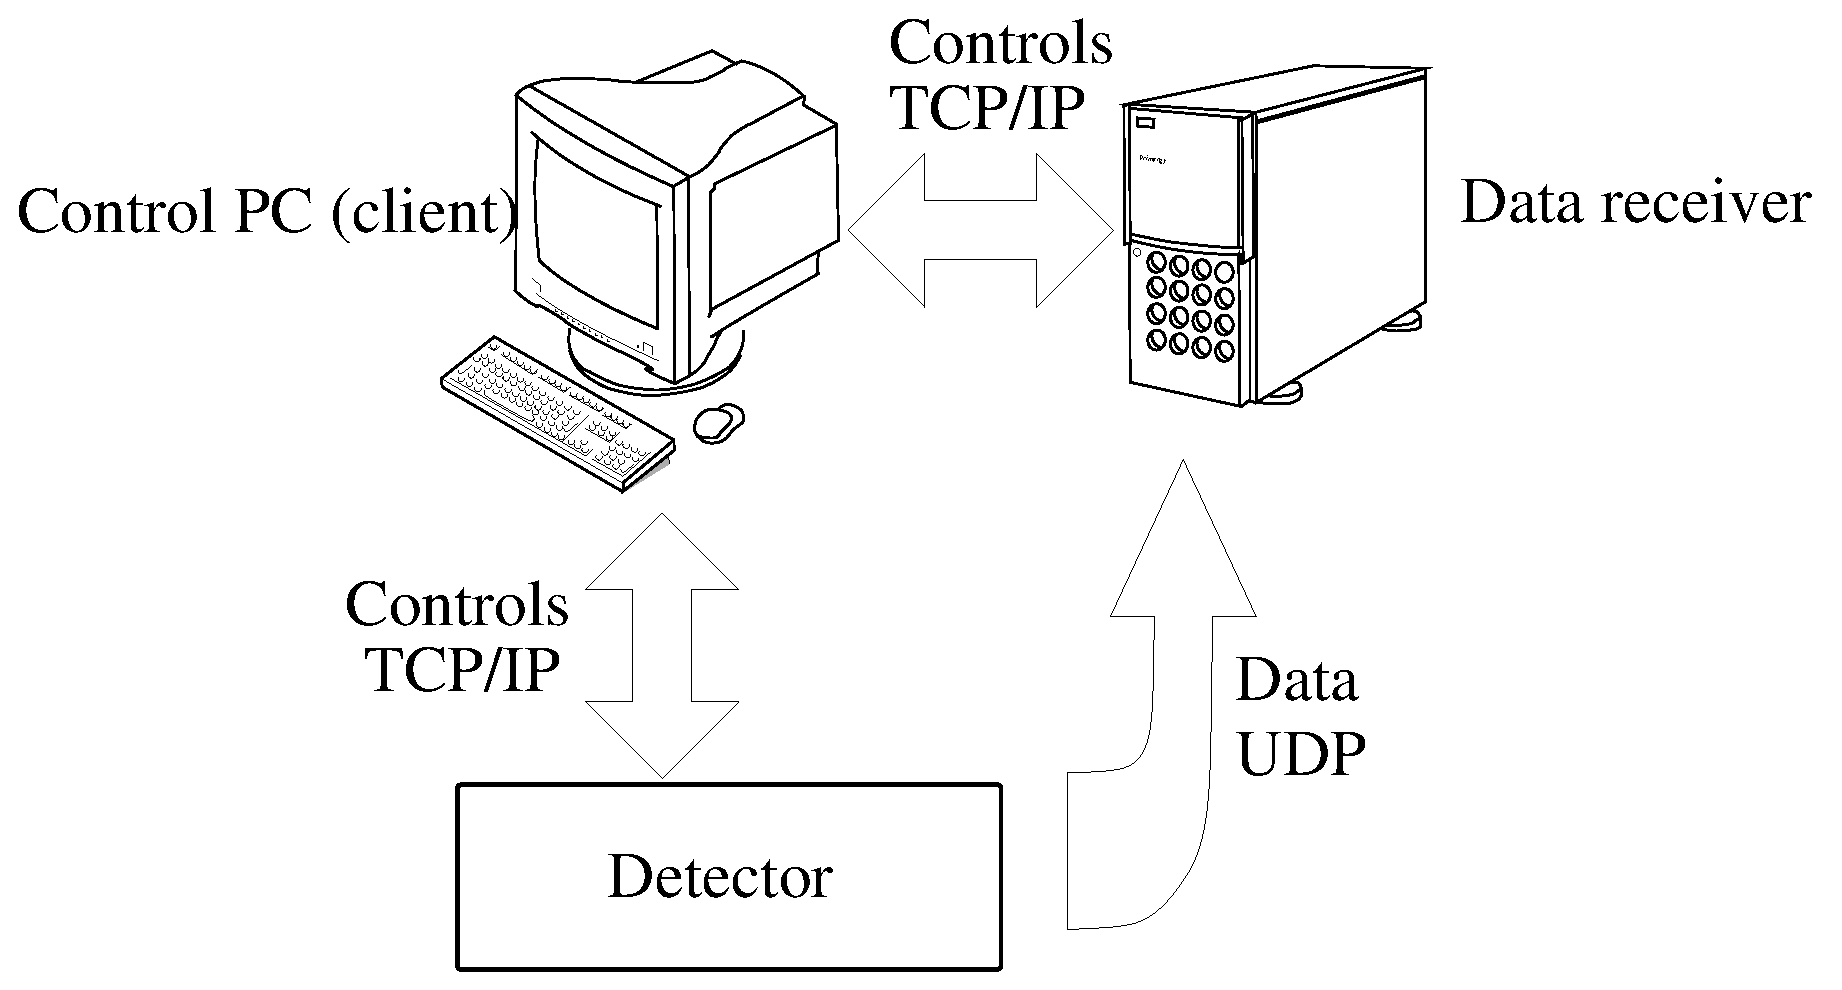
\includegraphics[width=\textwidth]{data_receiver}%
\lthtmlpictureZ
\lthtmlcheckvsize\clearpage}

\stepcounter{section}
\stepcounter{subsection}
\stepcounter{subsection}
\stepcounter{section}
\stepcounter{section}
{\newpage\clearpage
\lthtmlinlinemathA{tex2html_wrap_inline7759}%
$ d$%
\lthtmlinlinemathZ
\lthtmlcheckvsize\clearpage}

\stepcounter{section}
{\newpage\clearpage
\lthtmlinlinemathA{tex2html_wrap_inline7762}%
$ \Updownarrow$%
\lthtmlinlinemathZ
\lthtmlcheckvsize\clearpage}

{\newpage\clearpage
\lthtmlinlinemathA{tex2html_wrap_inline7764}%
$ \Rightarrow$%
\lthtmlinlinemathZ
\lthtmlcheckvsize\clearpage}

{\newpage\clearpage
\lthtmldisplayA{displaymath7766}%
\begin{displaymath}\textrm{\textbf{MEASUREMENTS}} \\
 \left\Updownarrow \,
    \begin{array}{l} \\
  %   \textrm{Measurement loop} \\
  \begin{array}{l} %\\
        	  \Rightarrow  \,  \textrm{Start script} \\
	   \\
\textrm{\textbf{SCAN0}}
           \left\Updownarrow 
     \,
	          \begin{array}{l} \\
                 	  \Rightarrow \,  \textrm{Scan0 script} \\
           %        \textrm{Scan 0 level} \\
		   \\
\par
\textrm{\textbf{SCAN1}}      \left\Updownarrow  
     \,
	          \begin{array}{l} \\
                %   \textrm{Scan 1 level} \\
		 \begin{array}{l} %\\
                 	  \Rightarrow \,  \textrm{Scan1 script} \\
                 	  \Rightarrow \,  \textrm{Script before} \\
		   \\
\begin{array}{l} \\
                    \textrm{\textbf{POSITIONS}} \left\Updownarrow  \,	  
\begin{array}{l} \\
             	  \Rightarrow \,     \textrm{Header before script} \\
		   \\
\par
\textrm{\textbf{CYCLES}}     \left\Updownarrow  \,
	          \begin{array}{l} \\
		  \\
\textrm{\textbf{FRAMES}}    \left\Updownarrow  \right. \\
		  \\
\\
		  \end{array}
		  \right. \\
		  \\
\Rightarrow \,  \textrm{Header after script}\\
		  \\
		  \end{array}
		  \right. \\
\\
\\
\\
           \end{array}
\par
\\
	 %  \\
\Rightarrow \, \textrm{Script after} \\
\end{array}
	  % \right. \\
	   \\
\\
                   \end{array}
	   \right. \\
\\
	   \\
\\
                   \end{array} 
	   \right. \\
	   \\
\Rightarrow	\,   \textrm{Stop script} \\
\\
            \end{array} 
 %     \right. \\
 \\
      \end{array}  
\right. 
\end{displaymath}%
\lthtmldisplayZ
\lthtmlcheckvsize\clearpage}

\stepcounter{section}
{\newpage\clearpage
\lthtmlpictureA{tex2html_wrap7789}%
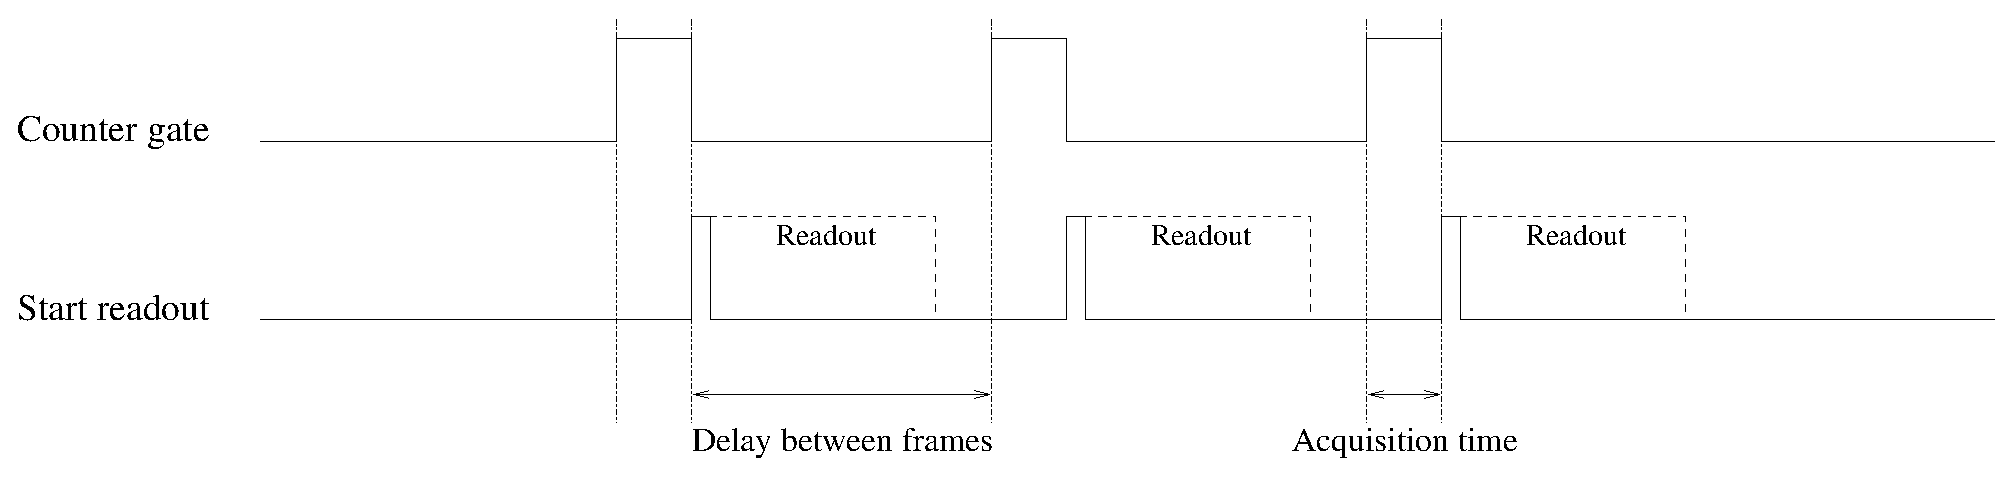
\includegraphics[width=\textwidth]{images/normal_acquisition.eps}%
\lthtmlpictureZ
\lthtmlcheckvsize\clearpage}

{\newpage\clearpage
\lthtmlpictureA{tex2html_wrap7793}%
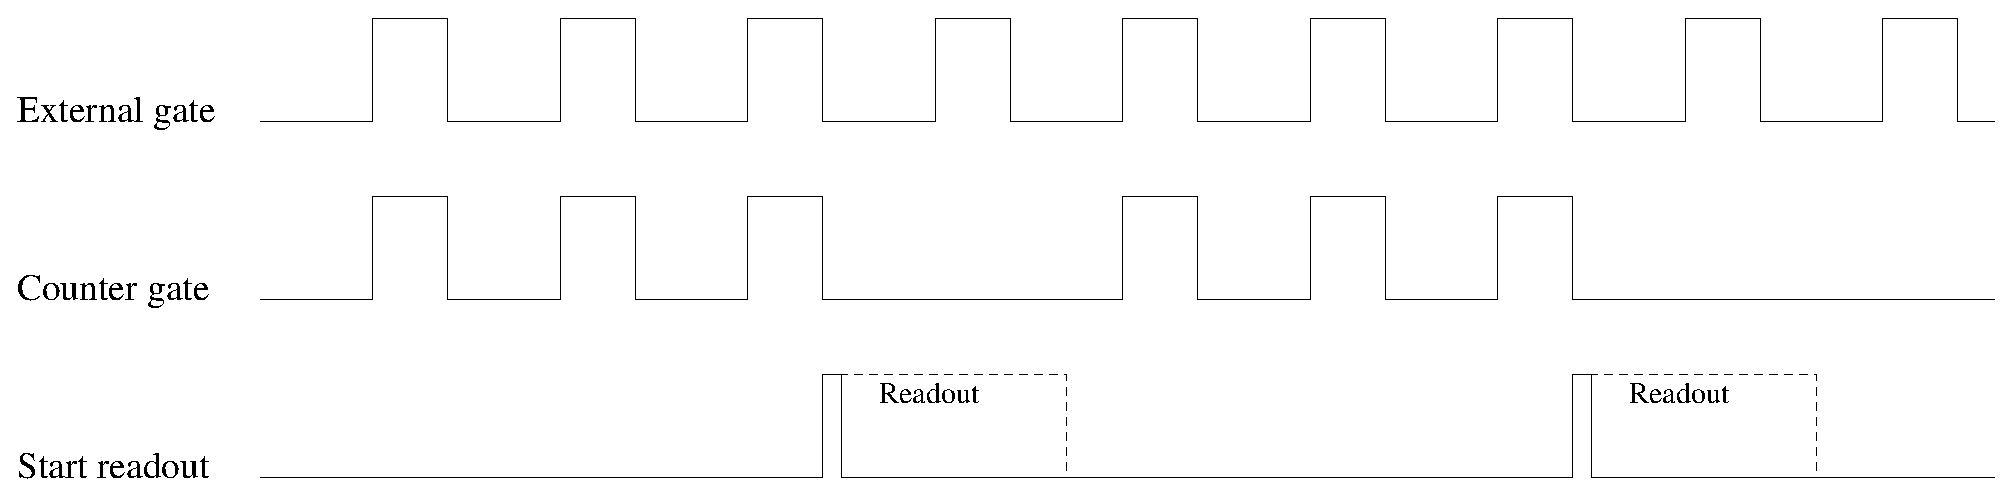
\includegraphics[width=\textwidth]{images/gated_acquisition.eps}%
\lthtmlpictureZ
\lthtmlcheckvsize\clearpage}

{\newpage\clearpage
\lthtmlpictureA{tex2html_wrap7797}%
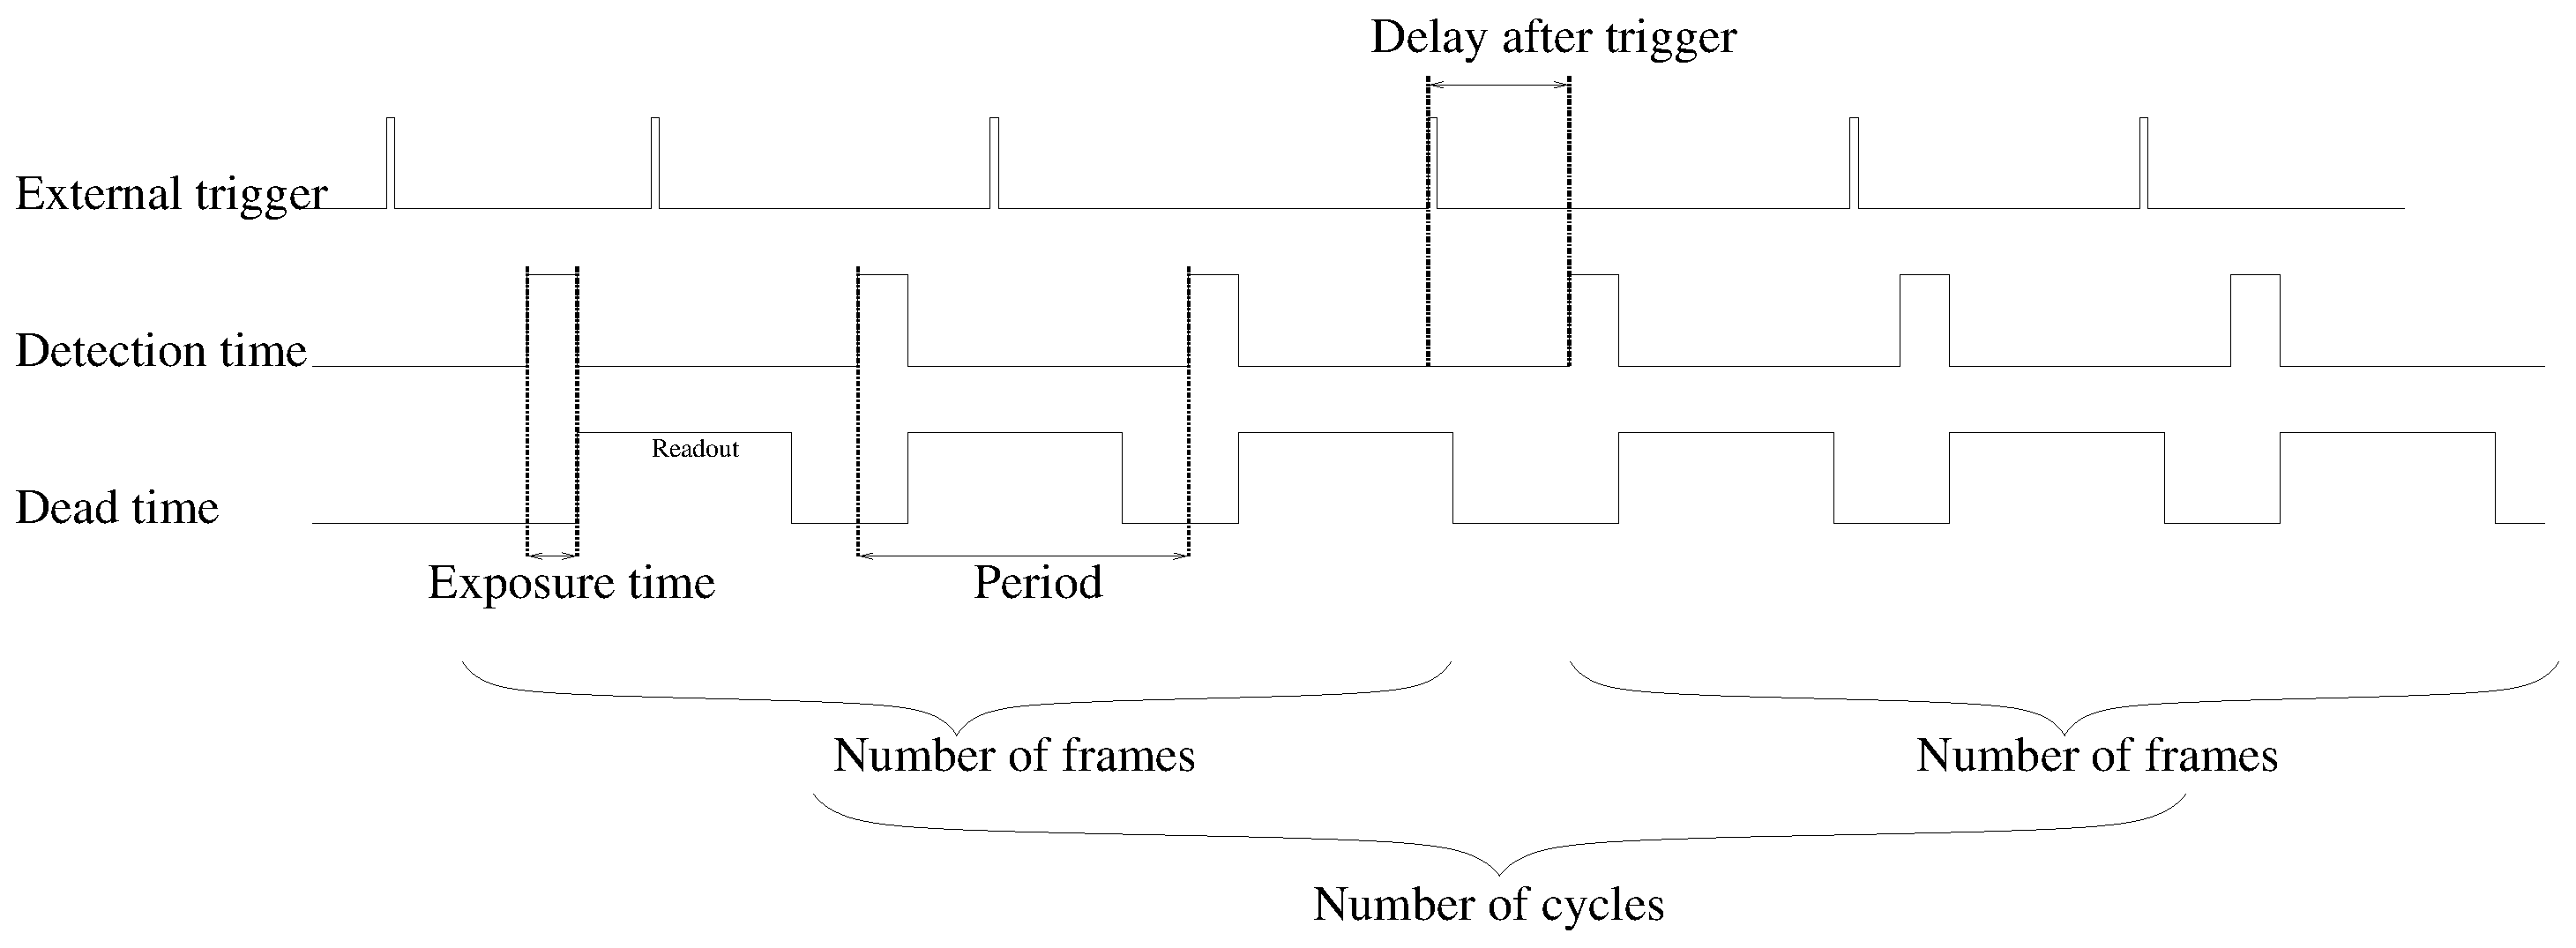
\includegraphics[width=\textwidth]{images/trigger_acquisition.eps}%
\lthtmlpictureZ
\lthtmlcheckvsize\clearpage}

{\newpage\clearpage
\lthtmlpictureA{tex2html_wrap7801}%
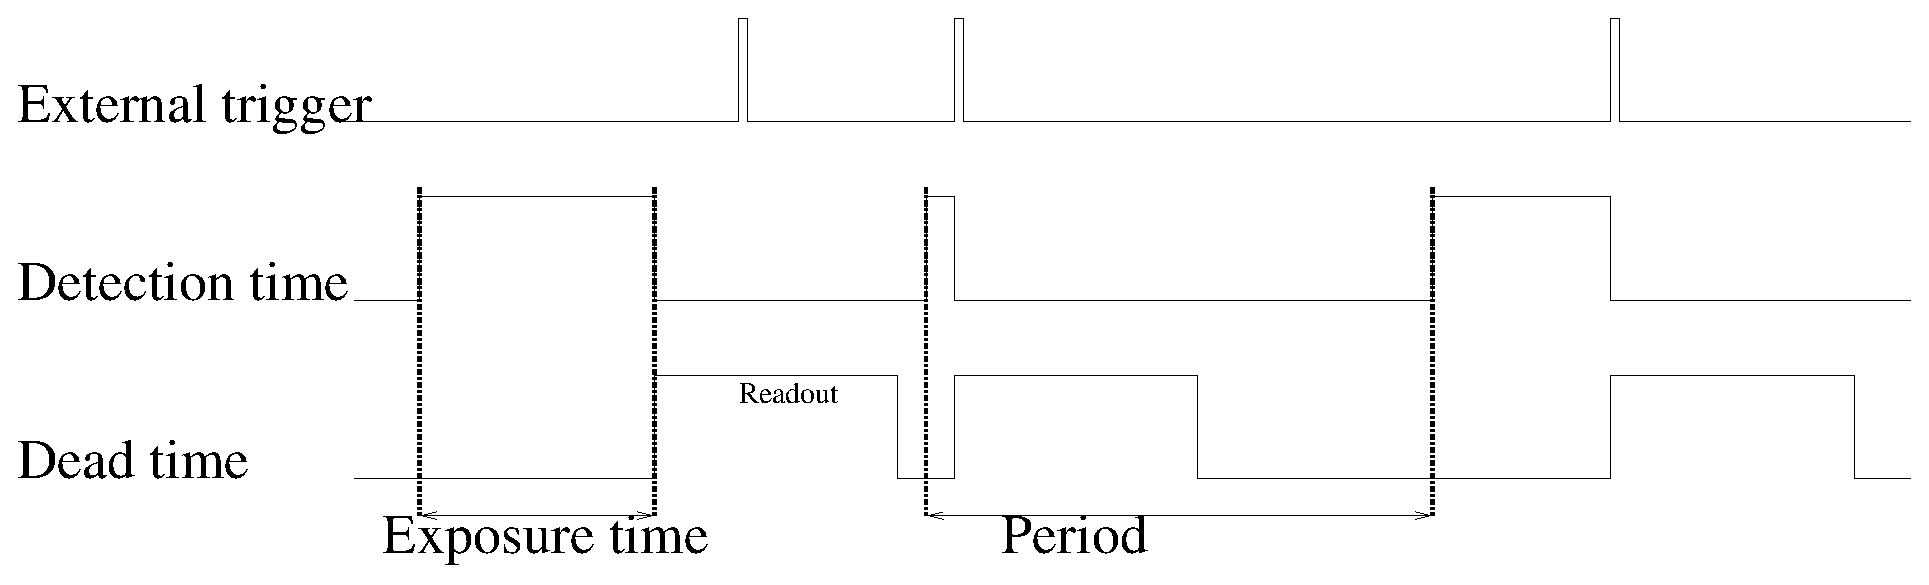
\includegraphics[width=\textwidth]{images/ro_trigger_acquisition.eps}%
\lthtmlpictureZ
\lthtmlcheckvsize\clearpage}

\stepcounter{section}
\stepcounter{section}
\stepcounter{section}
\stepcounter{subsection}
{\newpage\clearpage
\lthtmlinlinemathA{tex2html_wrap_inline7812}%
$ (108602\&0xFFFFFFFE)>>1 = 54301$%
\lthtmlinlinemathZ
\lthtmlcheckvsize\clearpage}

{\newpage\clearpage
\lthtmlinlinemathA{tex2html_wrap_inline7814}%
$ (108602\&0x1) =0$%
\lthtmlinlinemathZ
\lthtmlcheckvsize\clearpage}

\stepcounter{subsection}
\stepcounter{subsection}
\stepcounter{chapter}
\stepcounter{section}
\stepcounter{subsection}
{\newpage\clearpage
\lthtmlpictureA{tex2html_wrap7823}%
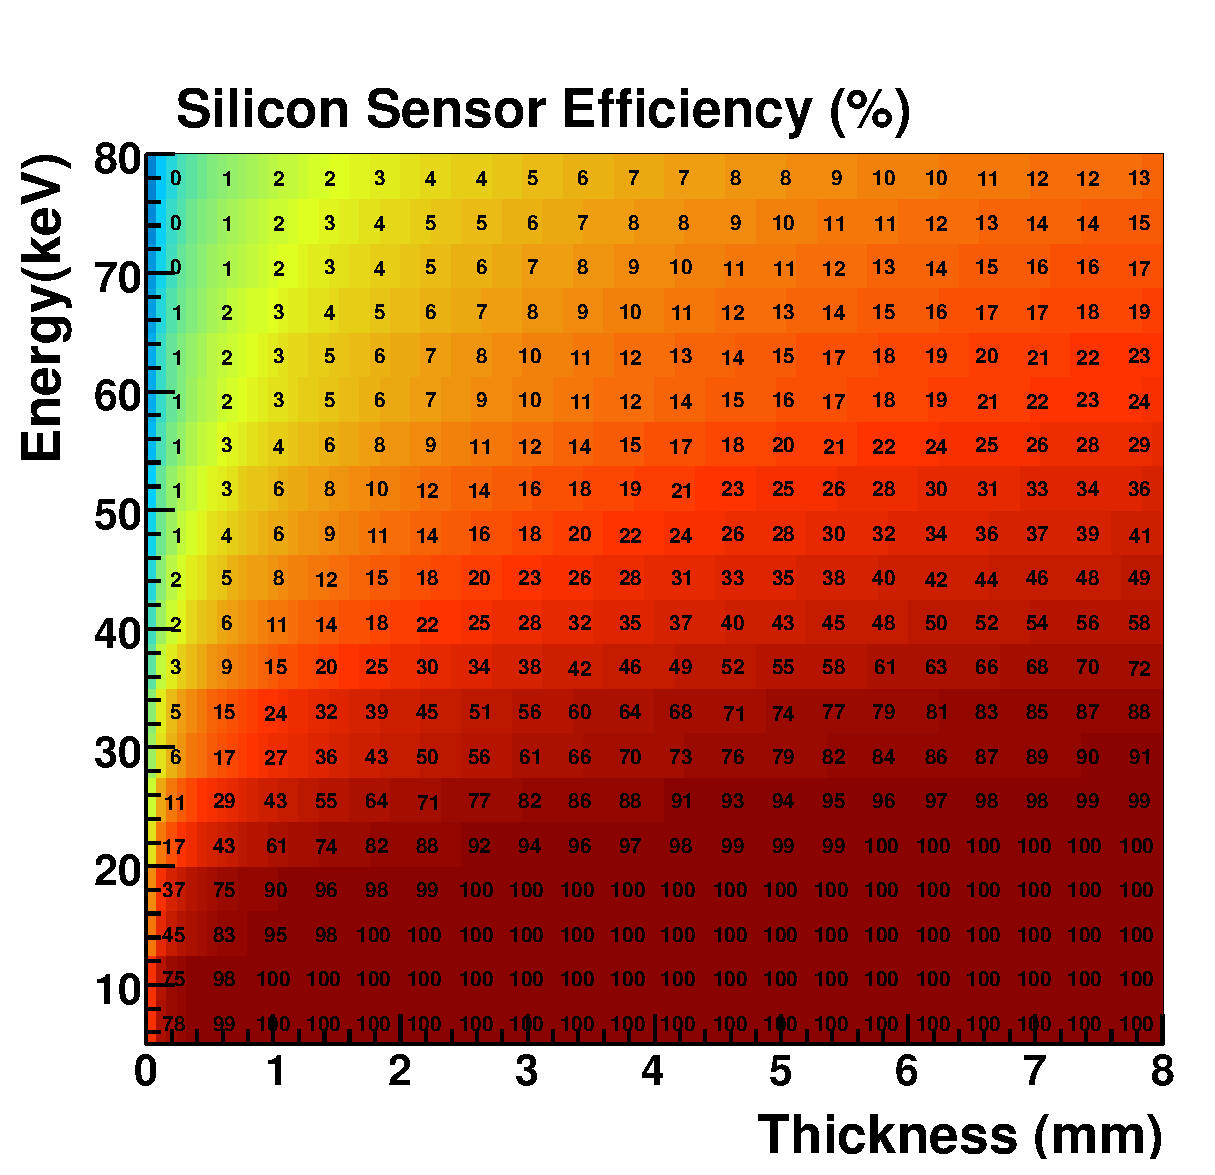
\includegraphics[width=\textwidth]{images/effiSiHardXRays2}%
\lthtmlpictureZ
\lthtmlcheckvsize\clearpage}

{\newpage\clearpage
\lthtmlinlinemathA{tex2html_wrap_inline7825}%
$ \mu$%
\lthtmlinlinemathZ
\lthtmlcheckvsize\clearpage}

{\newpage\clearpage
\lthtmlpictureA{tex2html_wrap7829}%
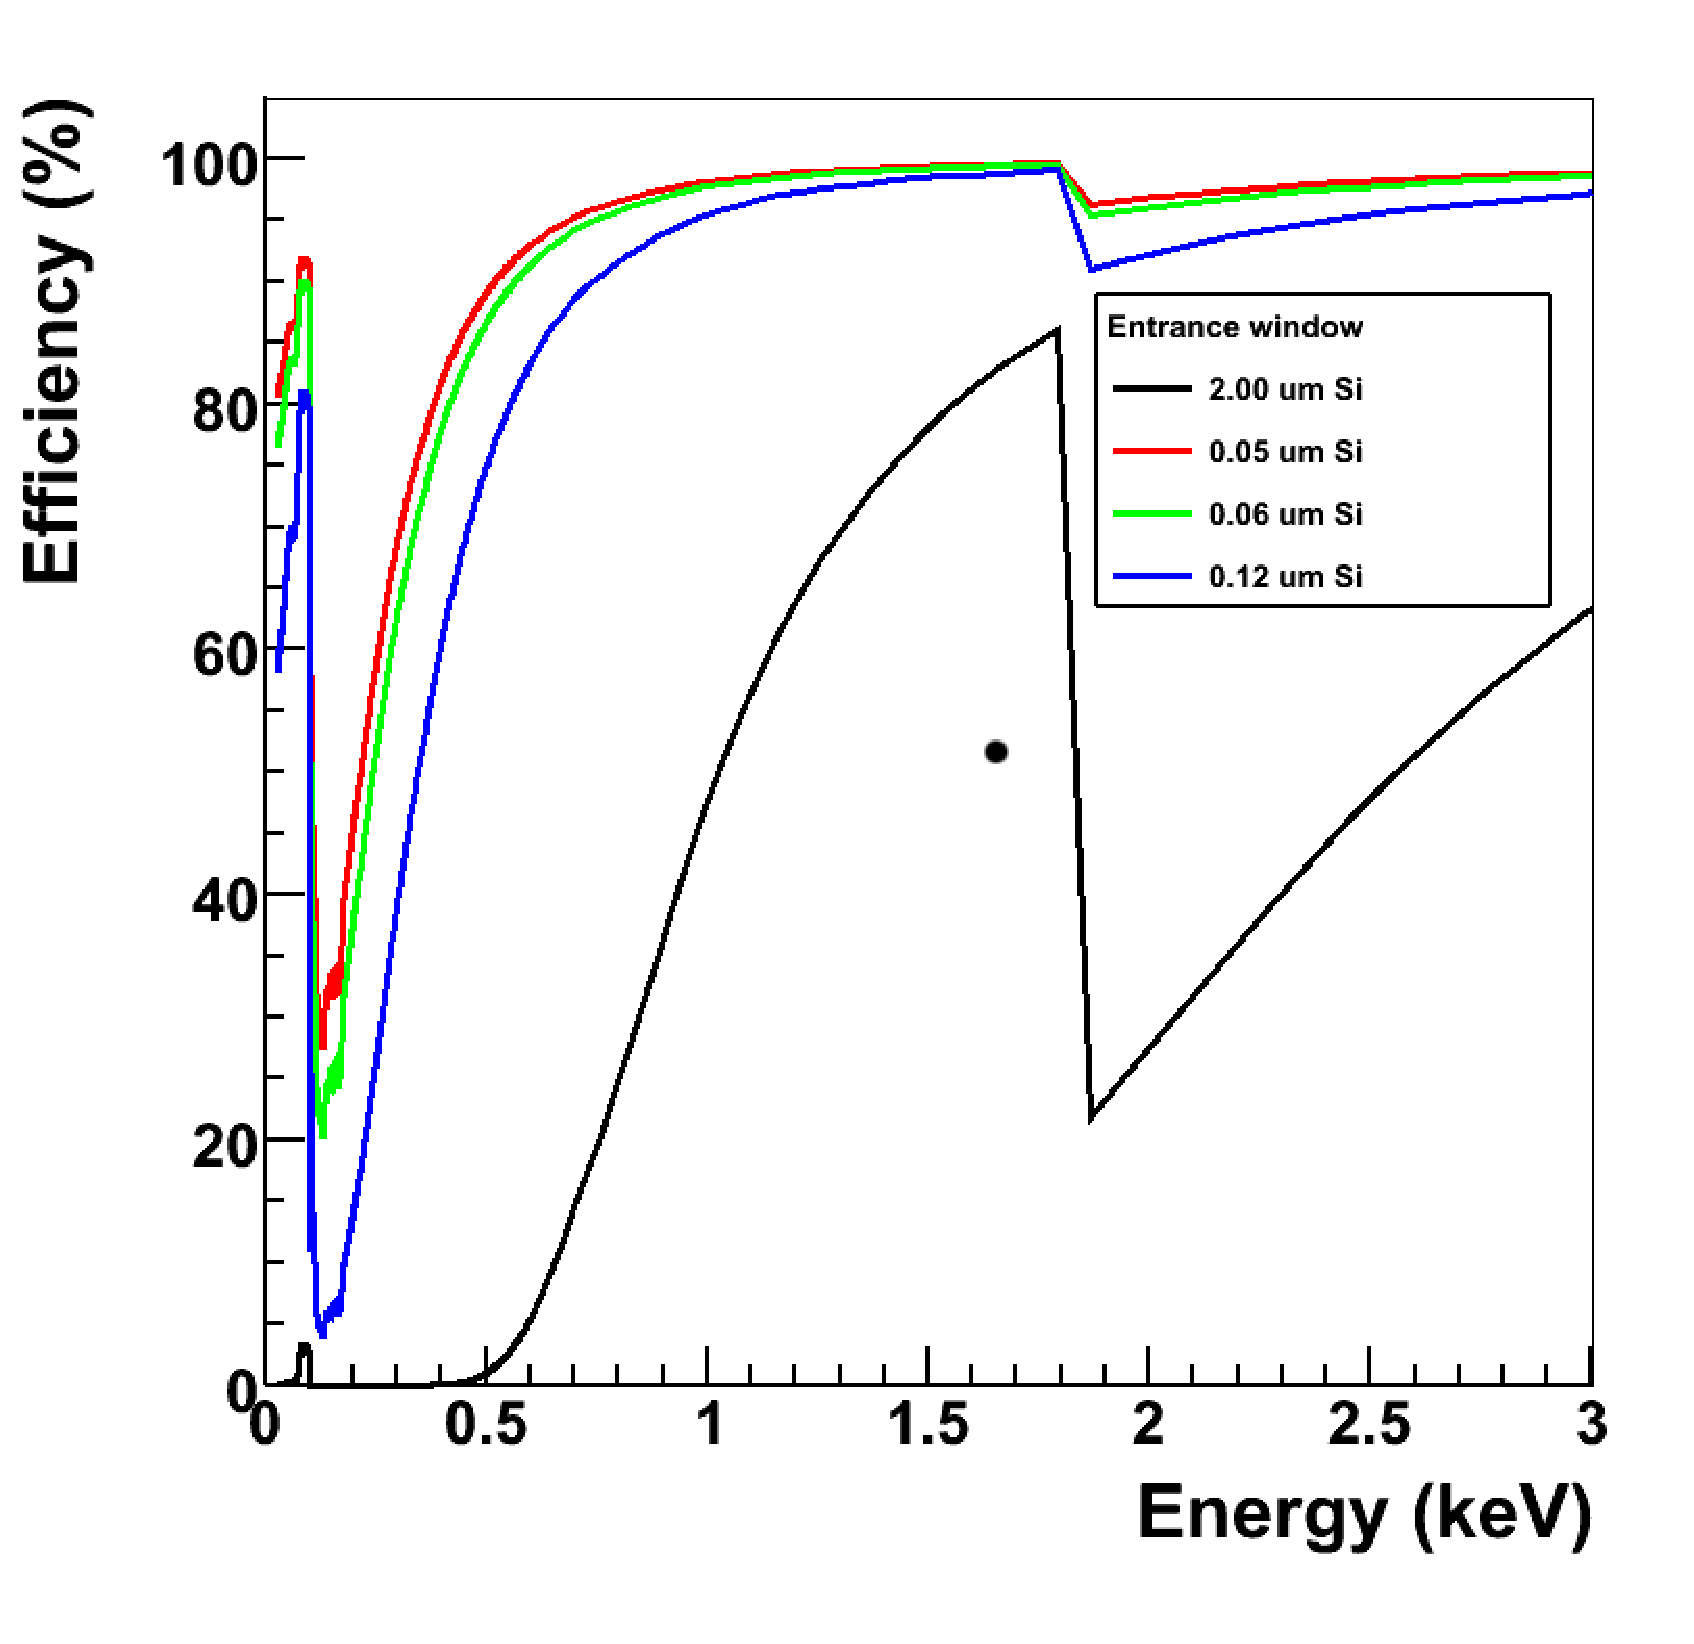
\includegraphics[width=\textwidth]{images/effiThinkBackplanes}%
\lthtmlpictureZ
\lthtmlcheckvsize\clearpage}

\stepcounter{subsection}
{\newpage\clearpage
\lthtmlpictureA{tex2html_wrap7834}%
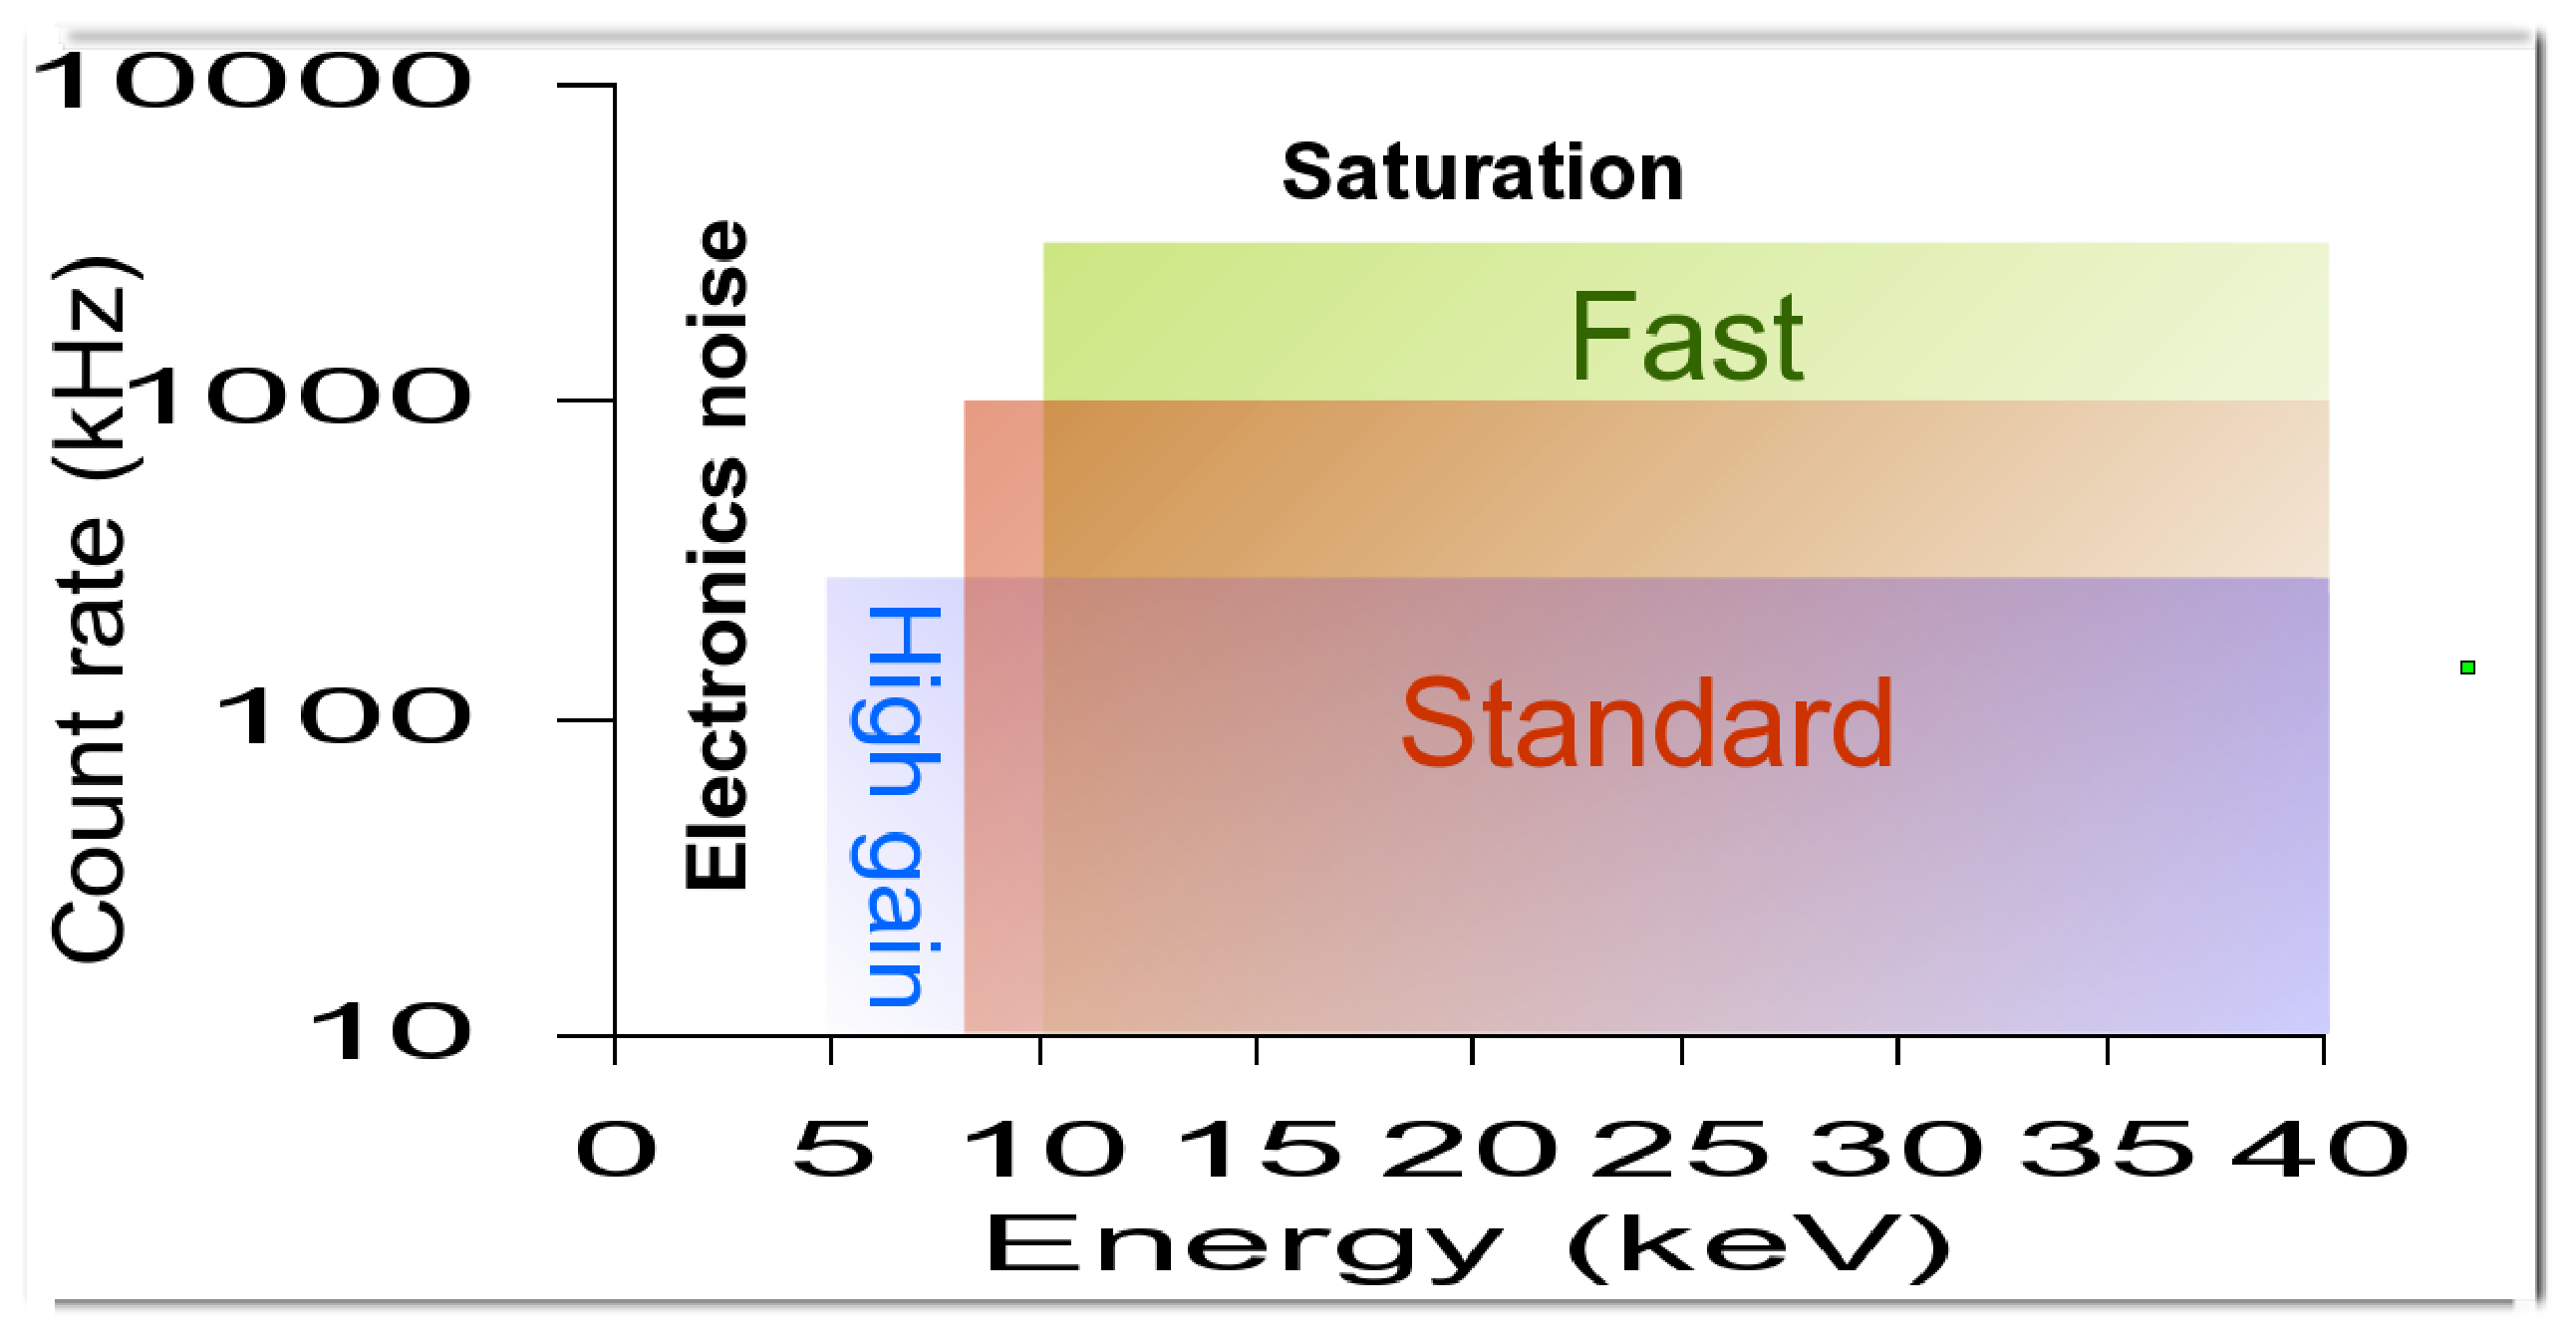
\includegraphics[width=\textwidth]{images/settings}%
\lthtmlpictureZ
\lthtmlcheckvsize\clearpage}

\stepcounter{section}
\stepcounter{chapter}
\stepcounter{section}
\stepcounter{subsection}
\stepcounter{section}
{\newpage\clearpage
\lthtmlpictureA{tex2html_wrap7844}%
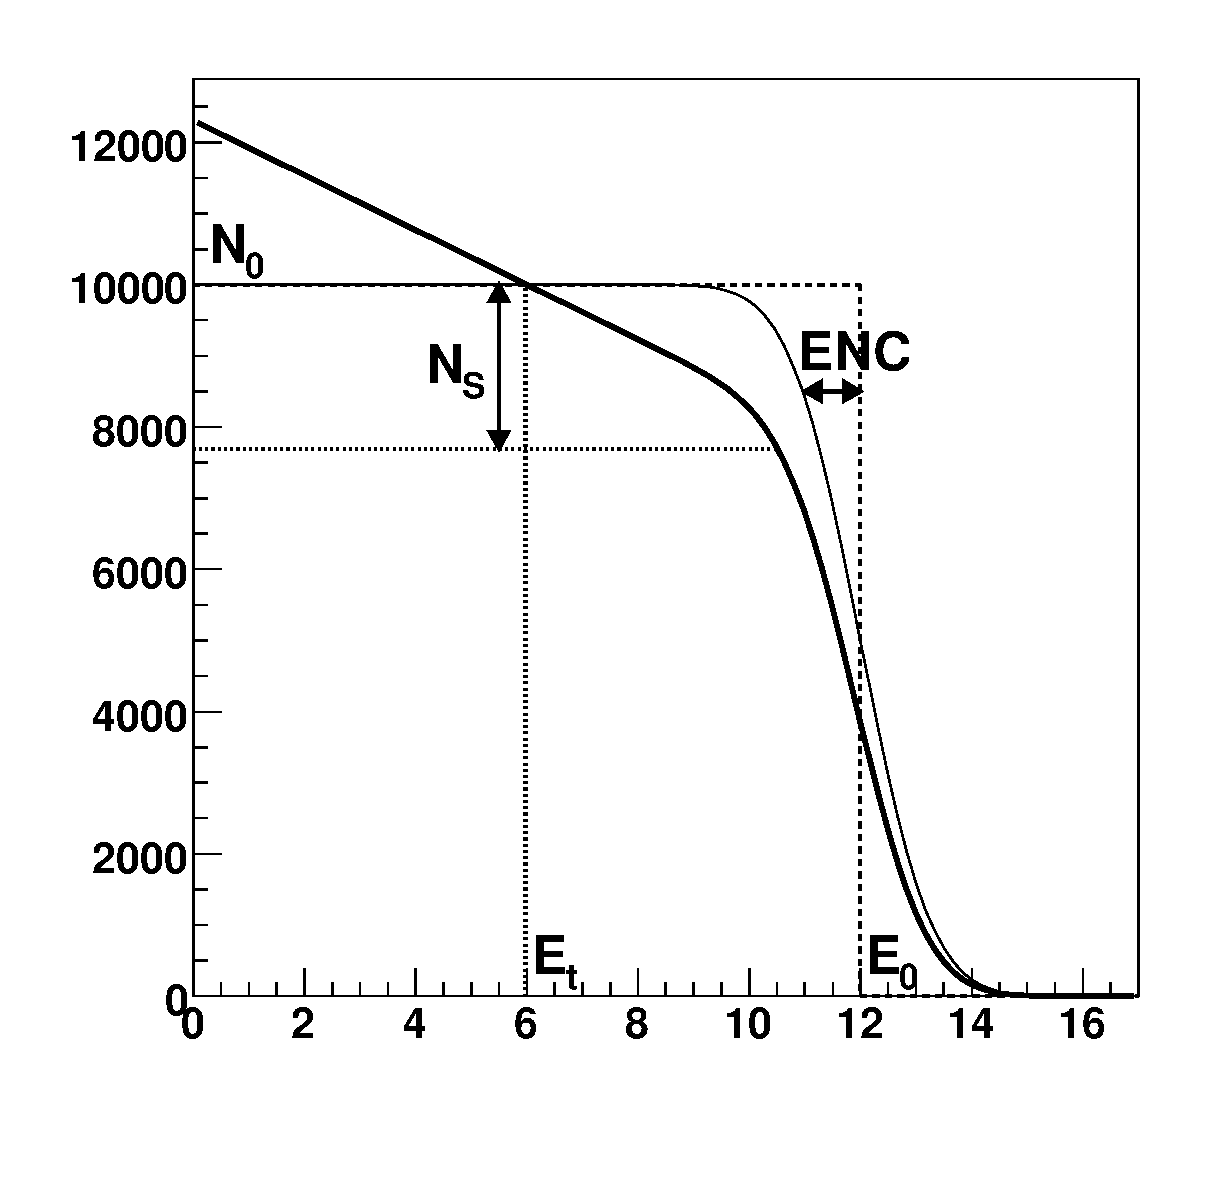
\includegraphics[width=\textwidth]{images/thr_scan_expl}%
\lthtmlpictureZ
\lthtmlcheckvsize\clearpage}

{\newpage\clearpage
\lthtmlpictureA{tex2html_wrap7848}%
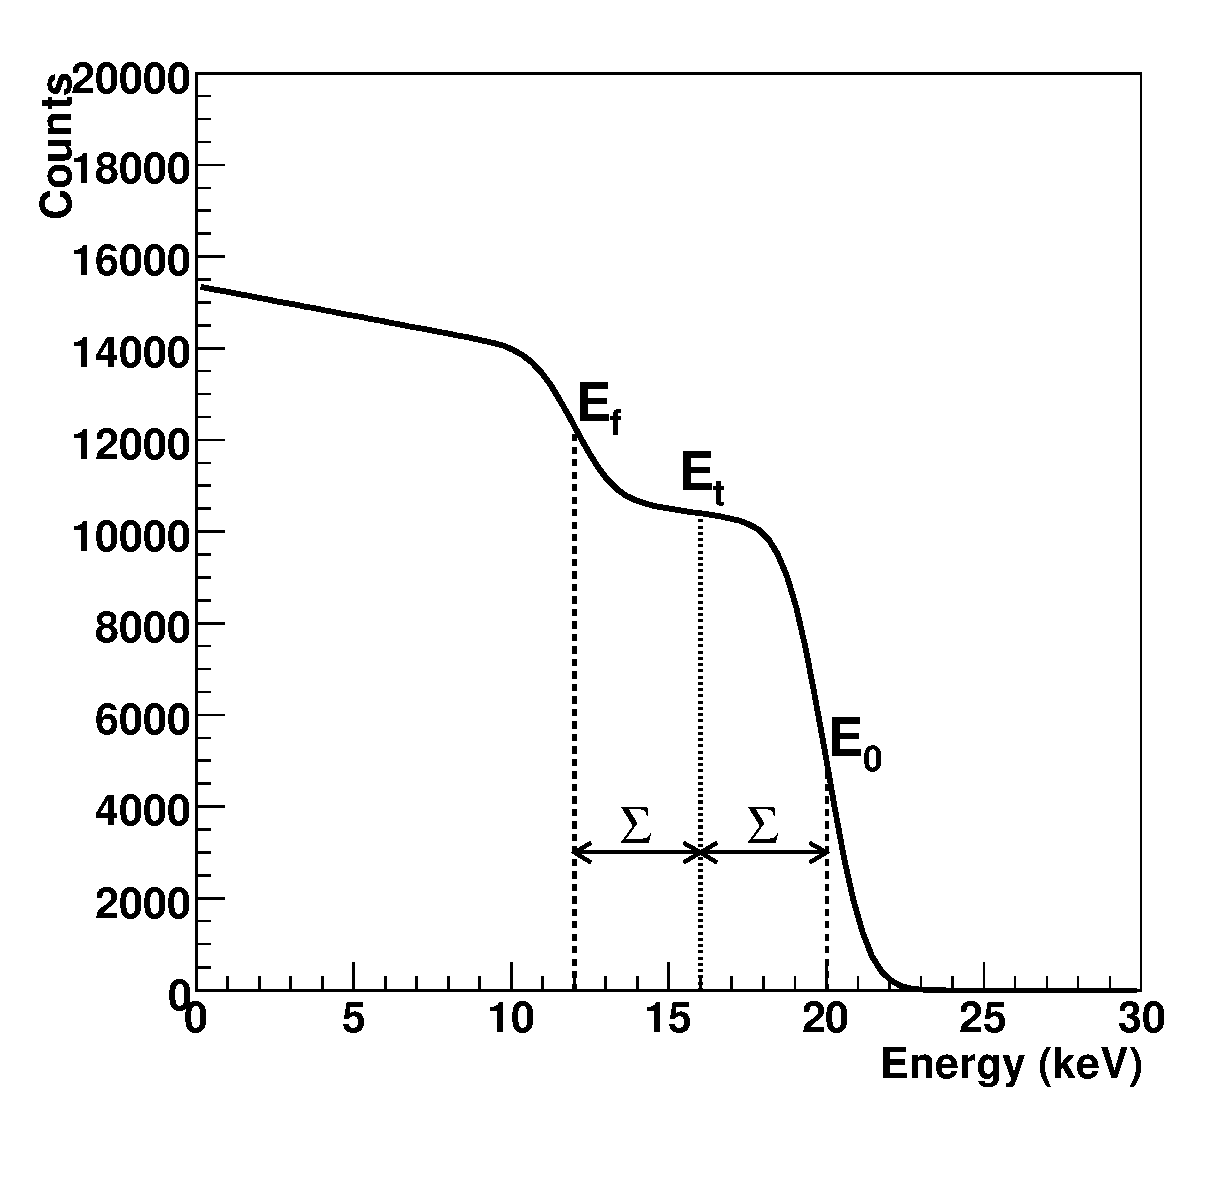
\includegraphics[width=\textwidth]{images/thr_scan_fluo}%
\lthtmlpictureZ
\lthtmlcheckvsize\clearpage}

{\newpage\clearpage
\lthtmlinlinemathA{tex2html_wrap_inline7853}%
$ E_0$%
\lthtmlinlinemathZ
\lthtmlcheckvsize\clearpage}

{\newpage\clearpage
\lthtmlinlinemathA{tex2html_wrap_inline7857}%
$ E_t=E_0/2$%
\lthtmlinlinemathZ
\lthtmlcheckvsize\clearpage}

{\newpage\clearpage
\lthtmlinlinemathA{tex2html_wrap_inline7861}%
$ E_f$%
\lthtmlinlinemathZ
\lthtmlcheckvsize\clearpage}

{\newpage\clearpage
\lthtmlinlinemathA{tex2html_wrap_inline7865}%
$ E_t$%
\lthtmlinlinemathZ
\lthtmlcheckvsize\clearpage}

{\newpage\clearpage
\lthtmlinlinemathA{tex2html_wrap_inline7879}%
$ E_f<E_0$%
\lthtmlinlinemathZ
\lthtmlcheckvsize\clearpage}

{\newpage\clearpage
\lthtmlinlinemathA{tex2html_wrap_inline7883}%
$ E_t>E_f+3$%
\lthtmlinlinemathZ
\lthtmlcheckvsize\clearpage}

{\newpage\clearpage
\lthtmlinlinemathA{tex2html_wrap_inline7885}%
$ E_t<E_0-3$%
\lthtmlinlinemathZ
\lthtmlcheckvsize\clearpage}

{\newpage\clearpage
\lthtmlinlinemathA{tex2html_wrap_inline7897}%
$ E_t<E_f-3$%
\lthtmlinlinemathZ
\lthtmlcheckvsize\clearpage}

{\newpage\clearpage
\lthtmlinlinemathA{tex2html_wrap_inline7901}%
$ E_t>4$%
\lthtmlinlinemathZ
\lthtmlcheckvsize\clearpage}

{\newpage\clearpage
\lthtmlpictureA{tex2html_wrap7908}%
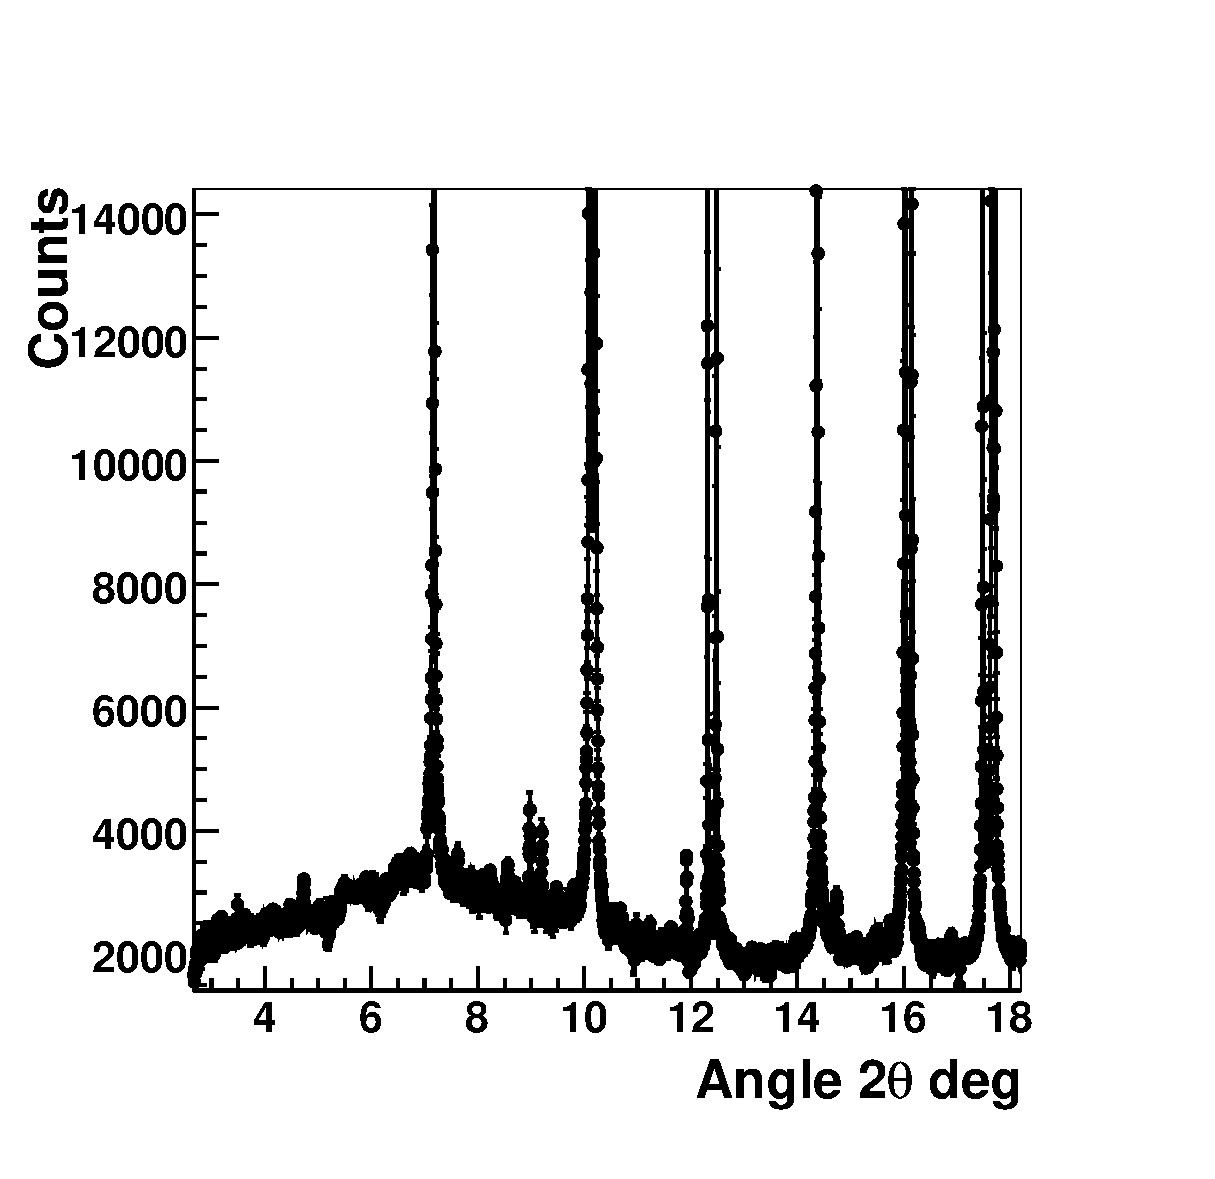
\includegraphics[width=\textwidth]{images/sample_with_fluorescence}%
\lthtmlpictureZ
\lthtmlcheckvsize\clearpage}

\stepcounter{section}
\stepcounter{subsection}
{\newpage\clearpage
\lthtmlpictureA{tex2html_wrap7914}%
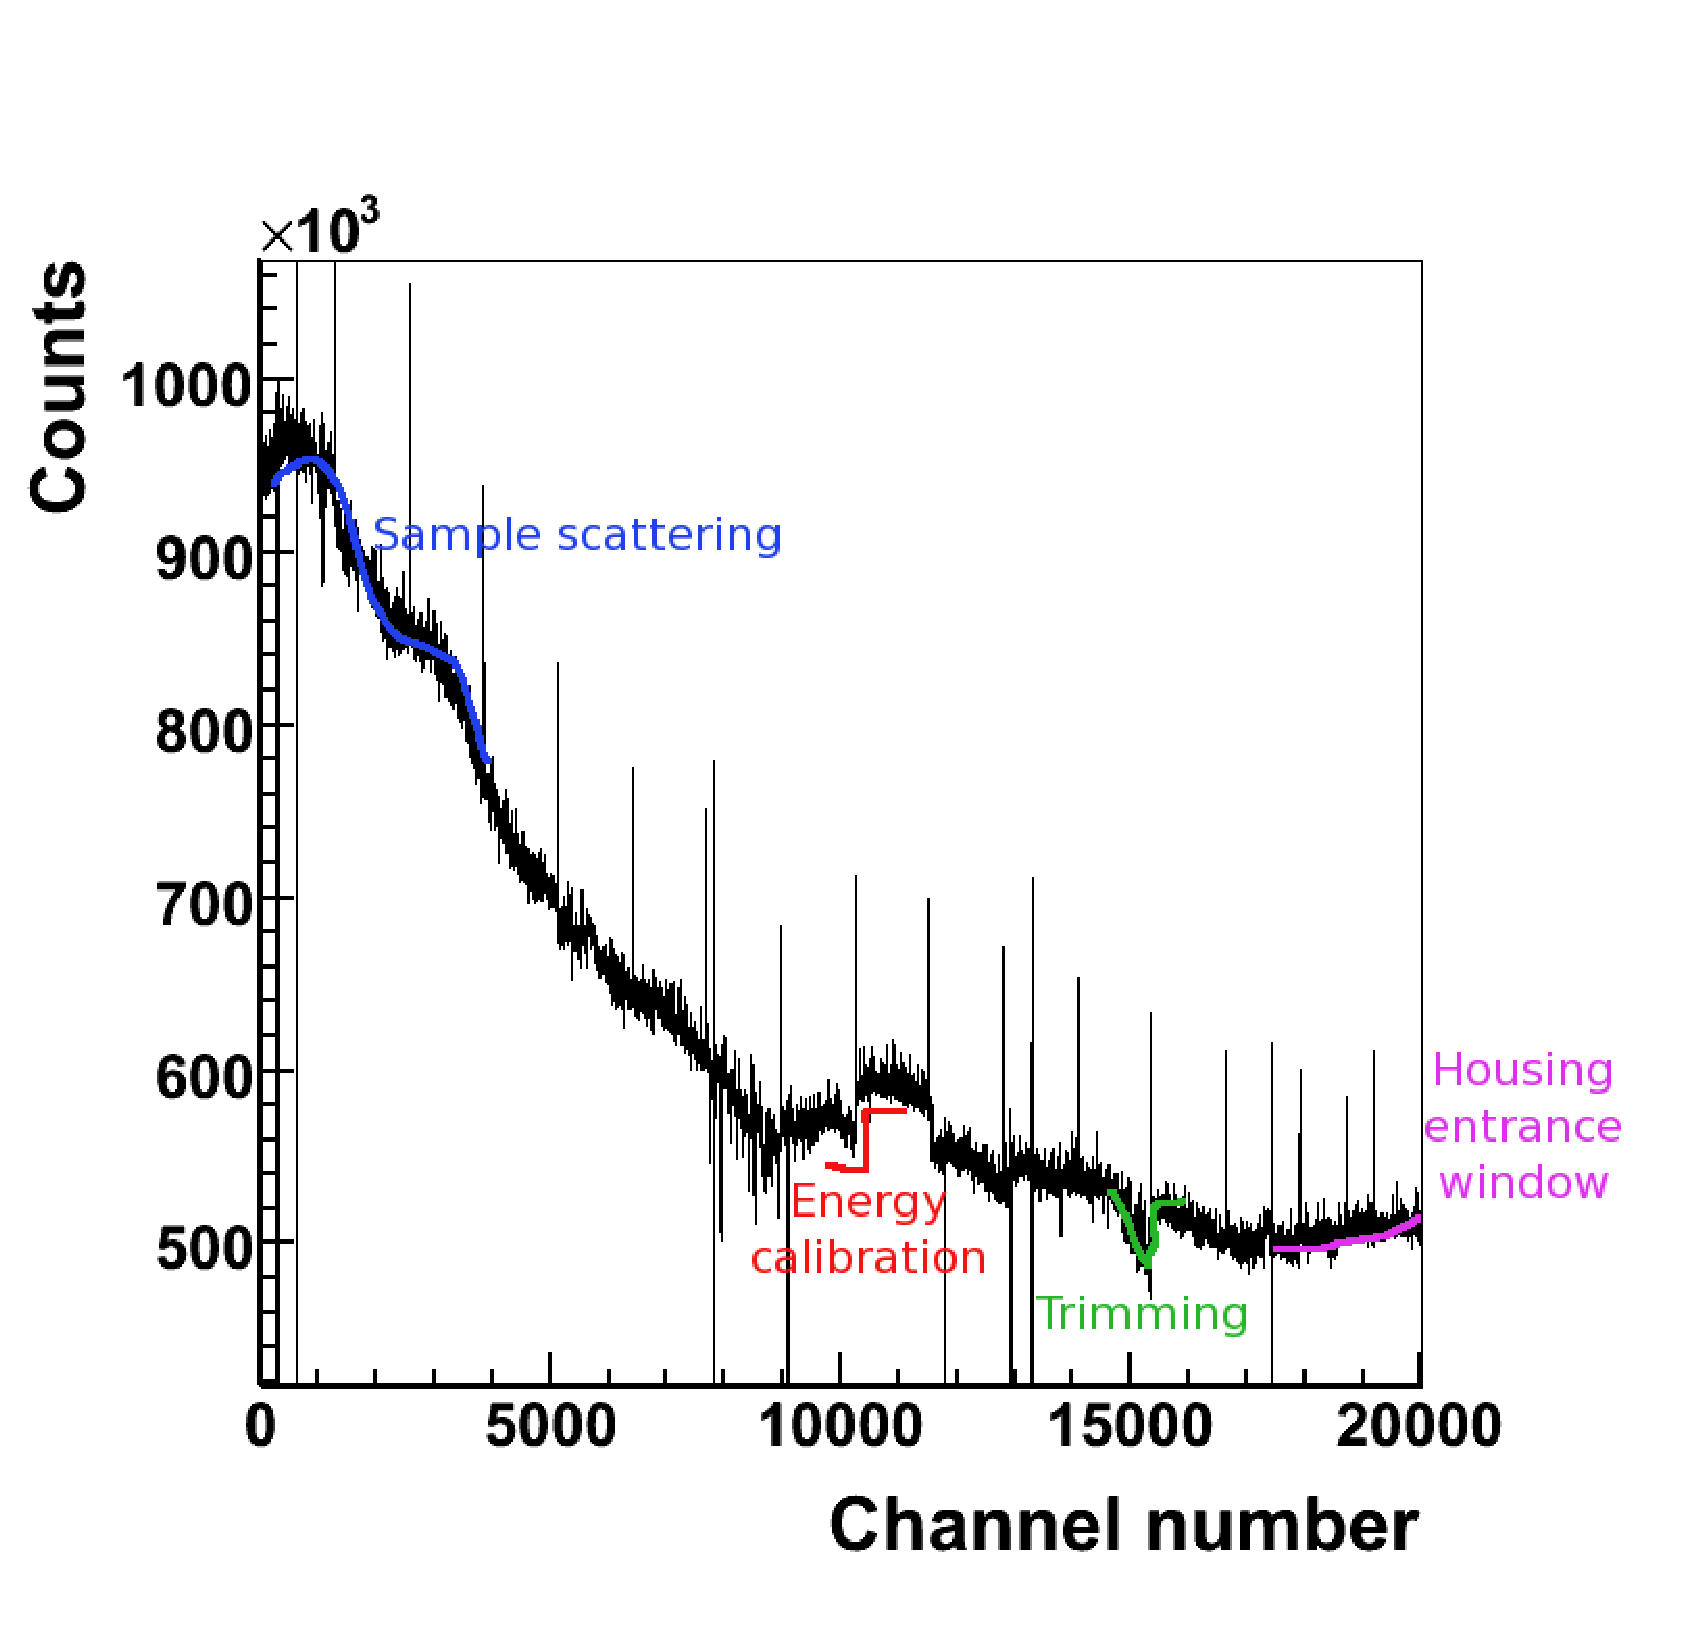
\includegraphics[width=\textwidth]{images/bad_ff_col}%
\lthtmlpictureZ
\lthtmlcheckvsize\clearpage}

\stepcounter{subsection}
{\newpage\clearpage
\lthtmlpictureA{tex2html_wrap7919}%
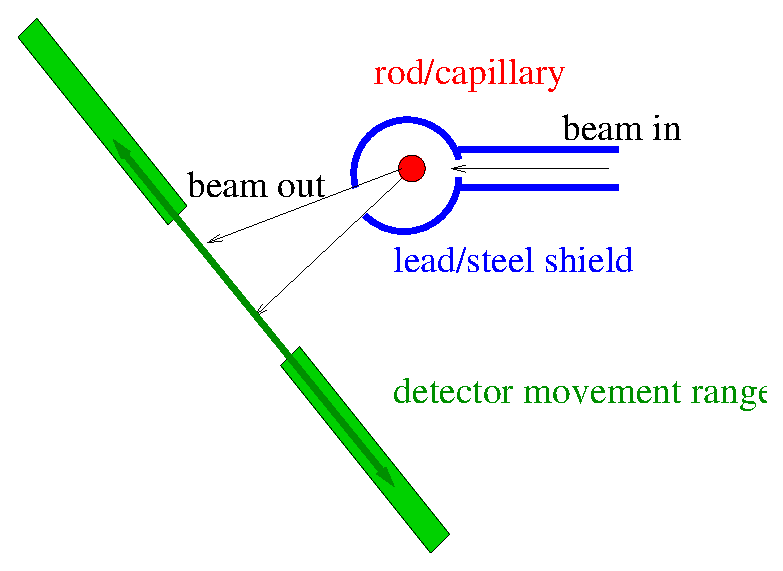
\includegraphics[width=\textwidth]{images/FFSetup}%
\lthtmlpictureZ
\lthtmlcheckvsize\clearpage}

\stepcounter{section}
\stepcounter{subsection}
{\newpage\clearpage
\lthtmlinlinemathA{tex2html_wrap_inline7926}%
$ Vthreshold=7$%
\lthtmlinlinemathZ
\lthtmlcheckvsize\clearpage}

{\newpage\clearpage
\lthtmlinlinemathA{tex2html_wrap_inline7928}%
$ Counts=500$%
\lthtmlinlinemathZ
\lthtmlcheckvsize\clearpage}

{\newpage\clearpage
\lthtmlinlinemathA{tex2html_wrap_inline7930}%
$ Resolution=4$%
\lthtmlinlinemathZ
\lthtmlcheckvsize\clearpage}

{\newpage\clearpage
\lthtmlinlinemathA{tex2html_wrap_inline7932}%
$ \pm$%
\lthtmlinlinemathZ
\lthtmlcheckvsize\clearpage}

{\newpage\clearpage
\lthtmlpictureA{tex2html_wrap7933}%
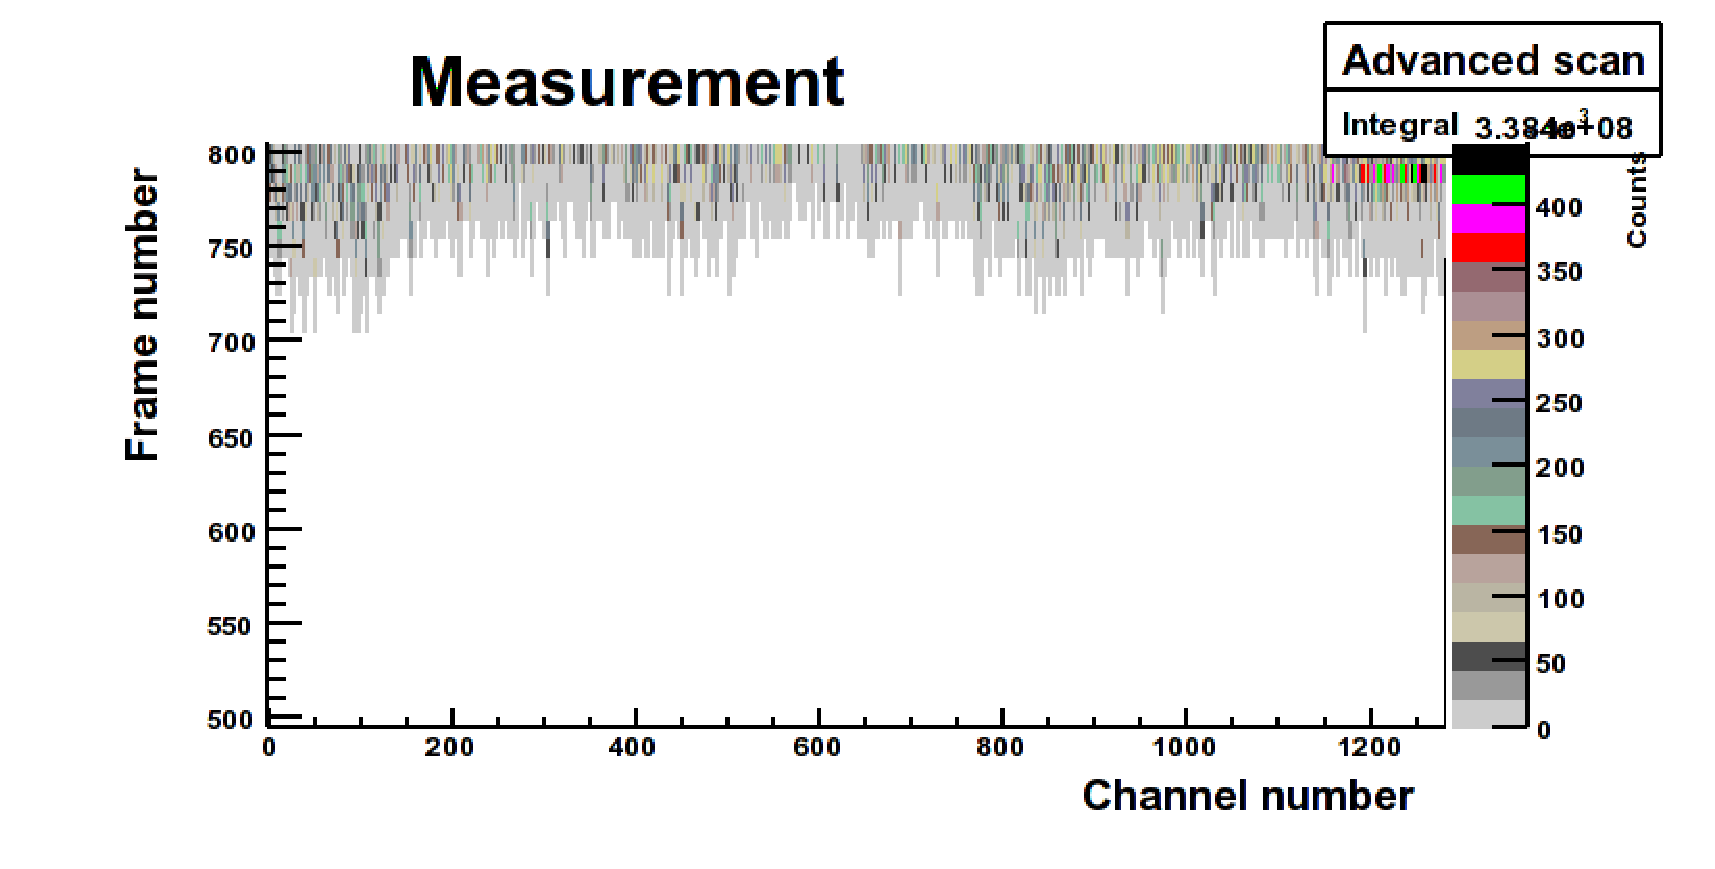
\includegraphics[width=\textwidth]{images/noise_thresholdscanuntrimmed}%
\lthtmlpictureZ
\lthtmlcheckvsize\clearpage}

{\newpage\clearpage
\lthtmlpictureA{tex2html_wrap7937}%
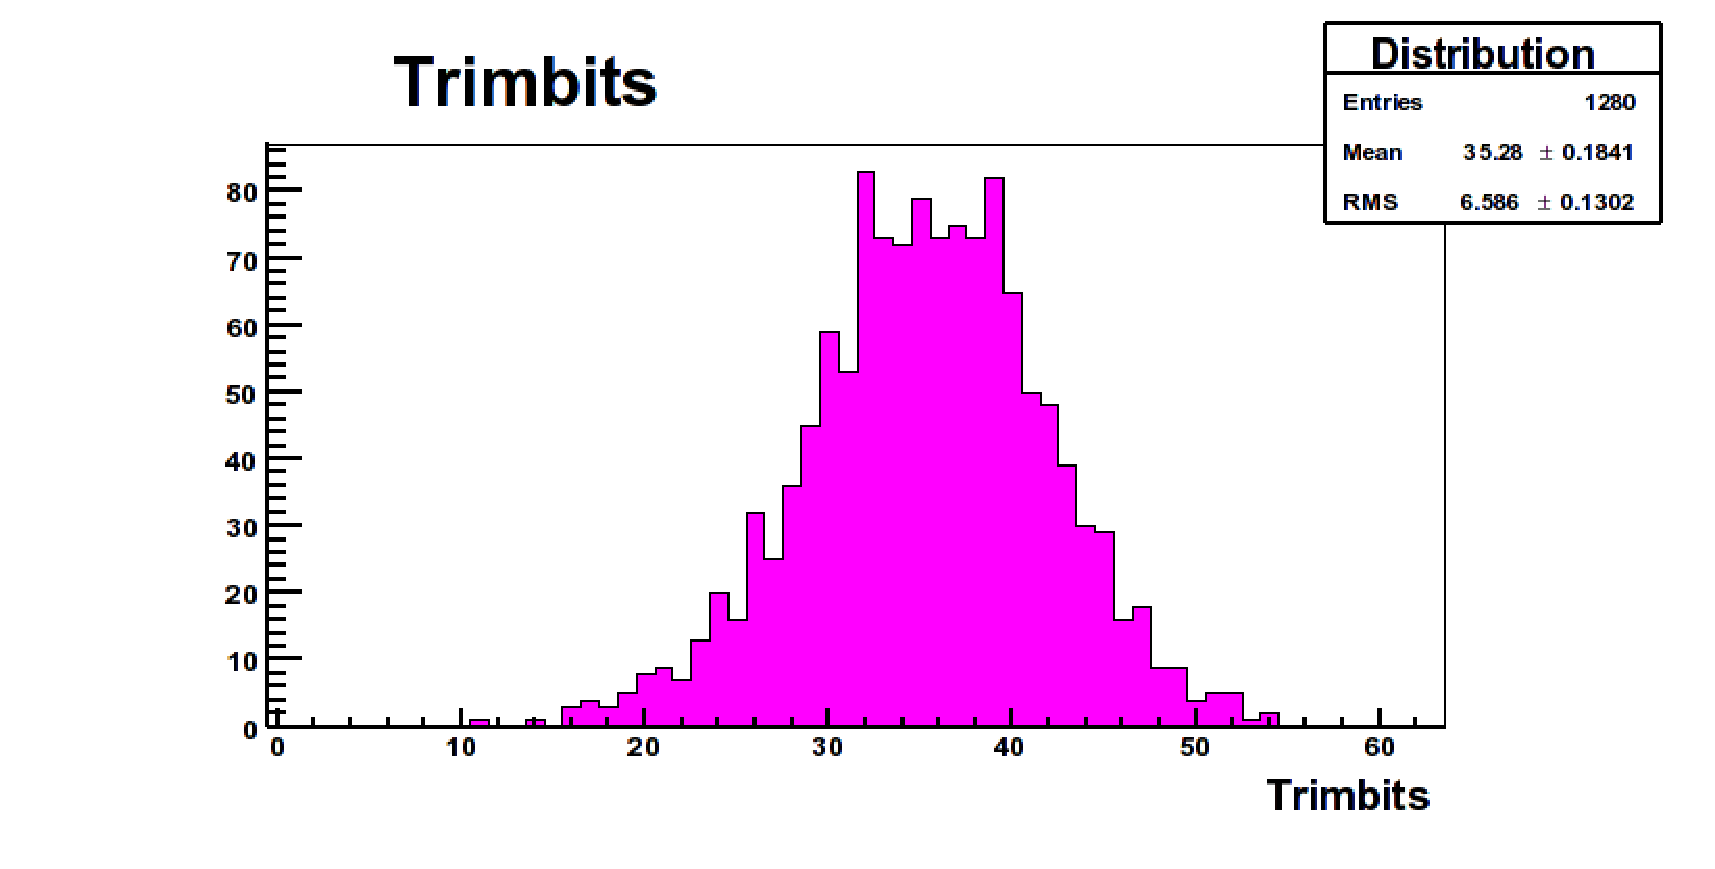
\includegraphics[width=\textwidth]{images/trimbitdistribution}%
\lthtmlpictureZ
\lthtmlcheckvsize\clearpage}

{\newpage\clearpage
\lthtmlpictureA{tex2html_wrap7941}%
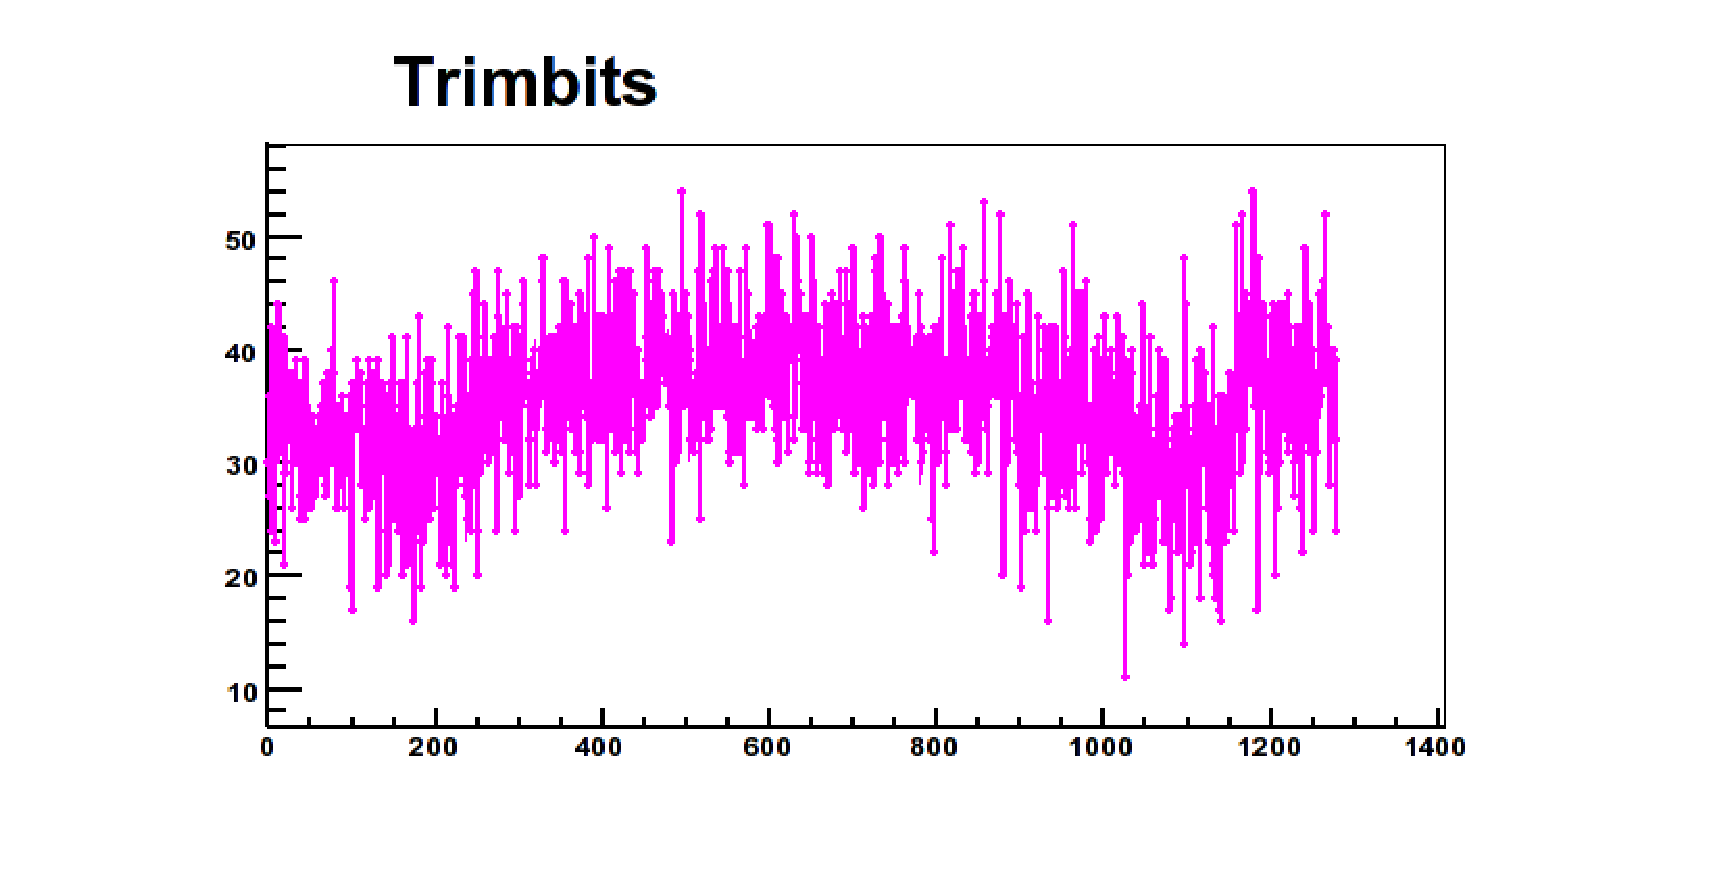
\includegraphics[width=\textwidth]{images/trimbitplot}%
\lthtmlpictureZ
\lthtmlcheckvsize\clearpage}

{\newpage\clearpage
\lthtmlpictureA{tex2html_wrap7945}%
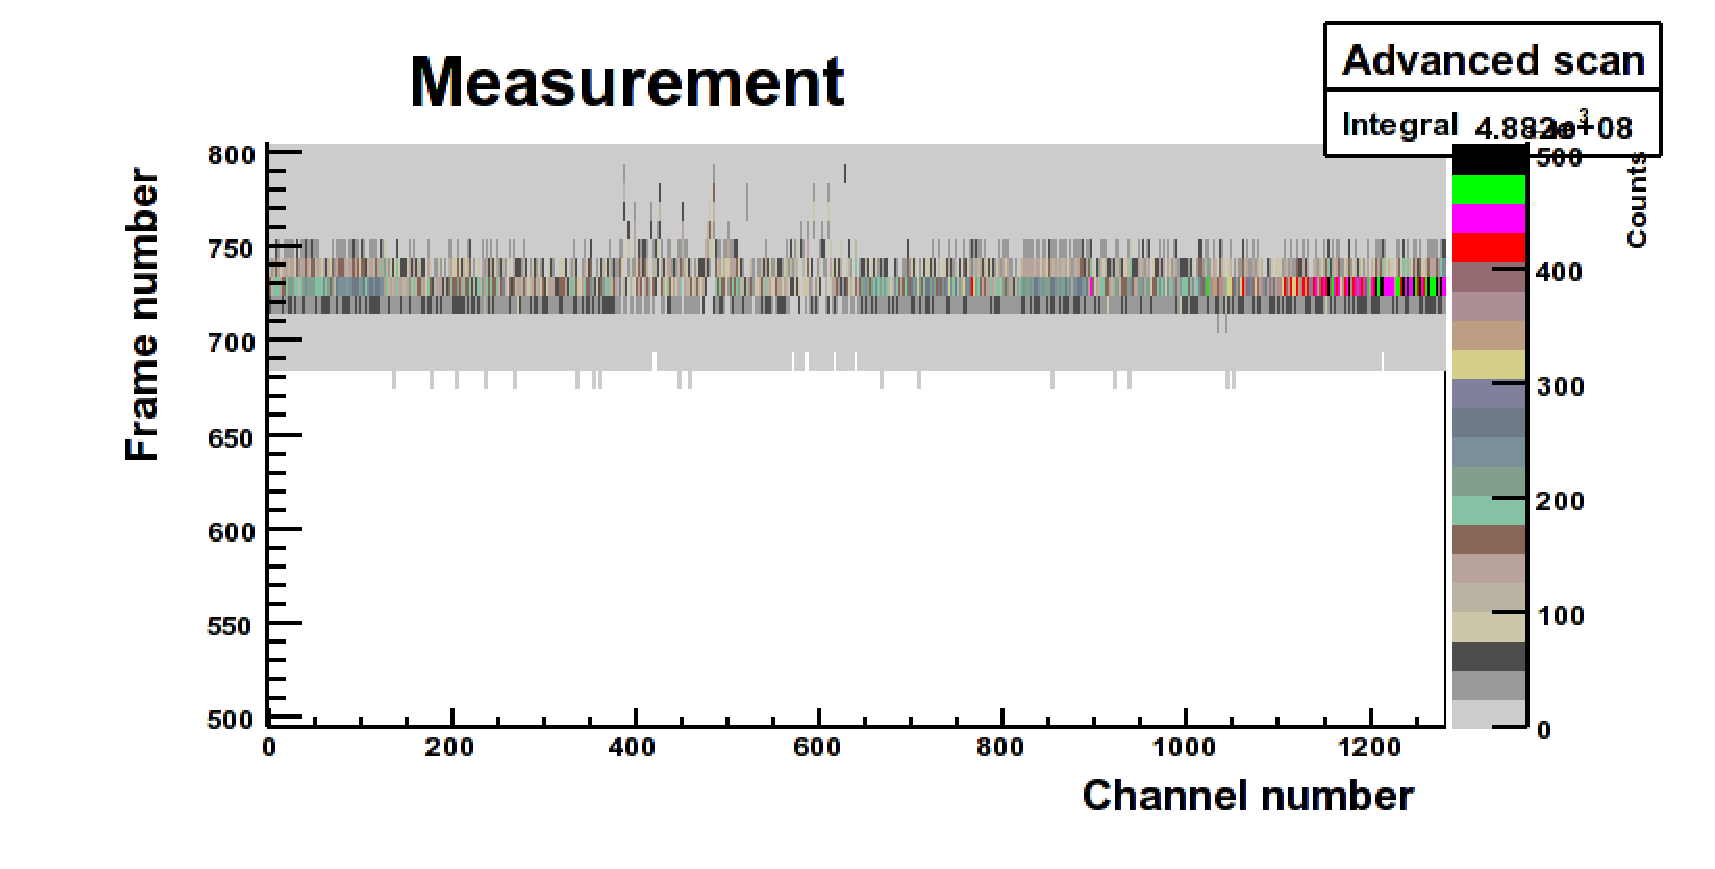
\includegraphics[width=\textwidth]{images/noise_thresholdscantrimmed}%
\lthtmlpictureZ
\lthtmlcheckvsize\clearpage}

\stepcounter{section}
\stepcounter{subsection}
{\newpage\clearpage
\lthtmlinlinemathA{tex2html_wrap_inline7954}%
$ \cdot$%
\lthtmlinlinemathZ
\lthtmlcheckvsize\clearpage}

\stepcounter{section}
\stepcounter{section}
\stepcounter{subsection}
\stepcounter{chapter}
\stepcounter{section}
\stepcounter{section}
\stepcounter{section}
\stepcounter{section}
\stepcounter{chapter}
\stepcounter{section}
{\newpage\clearpage
\lthtmlinlinemathA{tex2html_wrap_inline7968}%
$ \alpha_{jm}$%
\lthtmlinlinemathZ
\lthtmlcheckvsize\clearpage}

{\newpage\clearpage
\lthtmlinlinemathA{tex2html_wrap_inline7970}%
$ R_m$%
\lthtmlinlinemathZ
\lthtmlcheckvsize\clearpage}

{\newpage\clearpage
\lthtmlinlinemathA{tex2html_wrap_inline7972}%
$ \Phi_m$%
\lthtmlinlinemathZ
\lthtmlcheckvsize\clearpage}

{\newpage\clearpage
\lthtmlinlinemathA{tex2html_wrap_inline7974}%
$ D_m$%
\lthtmlinlinemathZ
\lthtmlcheckvsize\clearpage}

{\newpage\clearpage
\lthtmlinlinemathA{tex2html_wrap_inline7976}%
$ c_m$%
\lthtmlinlinemathZ
\lthtmlcheckvsize\clearpage}

{\newpage\clearpage
\lthtmlinlinemathA{tex2html_wrap_inline7978}%
$ o_m$%
\lthtmlinlinemathZ
\lthtmlcheckvsize\clearpage}

{\newpage\clearpage
\lthtmlinlinemathA{tex2html_wrap_inline7980}%
$ k_m$%
\lthtmlinlinemathZ
\lthtmlcheckvsize\clearpage}

{\newpage\clearpage
\lthtmlinlinemathA{tex2html_wrap_indisplay7982}%
$\displaystyle \alpha_{jm}=\Phi_m-{\ensuremath{\left({{\ensuremath{\displaystyle{\frac{{\ensuremath{\displaystyle{180}}}}{{\ensuremath{\displaystyle{\pi}}}}}}}}\right)}}\arctan{\ensuremath{\left({{\ensuremath{\displaystyle{\frac{{\ensuremath{\displaystyle{D_m-pj}}}}{{\ensuremath{\displaystyle{R_m}}}}}}}}\right)}}$%
\lthtmlindisplaymathZ
\lthtmlcheckvsize\clearpage}

{\newpage\clearpage
\lthtmlinlinemathA{tex2html_wrap_indisplay7984}%
$\displaystyle \alpha_{jm}=o_m+{\ensuremath{\left({{\ensuremath{\displaystyle{\frac{{\ensuremath{\displaystyle{180}}}}{{\ensuremath{\displaystyle{\pi}}}}}}}}\right)}}c_mk_m+{\ensuremath{\left({{\ensuremath{\displaystyle{\frac{{\ensuremath{\displaystyle{180}}}}{{\ensuremath{\displaystyle{\pi}}}}}}}}\right)}}\arctan{\ensuremath{\left[{{\ensuremath{\left({j-c_m}\right)}}k_m}\right]}}$%
\lthtmlindisplaymathZ
\lthtmlcheckvsize\clearpage}

{\newpage\clearpage
\lthtmlinlinemathA{tex2html_wrap_indisplay7987}%
$\displaystyle c_m$%
\lthtmlindisplaymathZ
\lthtmlcheckvsize\clearpage}

{\newpage\clearpage
\lthtmlinlinemathA{tex2html_wrap_indisplay7989}%
$\displaystyle =$%
\lthtmlindisplaymathZ
\lthtmlcheckvsize\clearpage}

{\newpage\clearpage
\lthtmlinlinemathA{tex2html_wrap_indisplay7991}%
$\displaystyle {\ensuremath{\displaystyle{\frac{{\ensuremath{\displaystyle{D_m}}}}{{\ensuremath{\displaystyle{p}}}}}}};$%
\lthtmlindisplaymathZ
\lthtmlcheckvsize\clearpage}

{\newpage\clearpage
\lthtmlinlinemathA{tex2html_wrap_indisplay7993}%
$\displaystyle k_m$%
\lthtmlindisplaymathZ
\lthtmlcheckvsize\clearpage}

{\newpage\clearpage
\lthtmlinlinemathA{tex2html_wrap_indisplay7997}%
$\displaystyle {\ensuremath{\displaystyle{\frac{{\ensuremath{\displaystyle{p}}}}{{\ensuremath{\displaystyle{R_m}}}}}}};$%
\lthtmlindisplaymathZ
\lthtmlcheckvsize\clearpage}

{\newpage\clearpage
\lthtmlinlinemathA{tex2html_wrap_indisplay7999}%
$\displaystyle o_m$%
\lthtmlindisplaymathZ
\lthtmlcheckvsize\clearpage}

{\newpage\clearpage
\lthtmlinlinemathA{tex2html_wrap_indisplay8003}%
$\displaystyle \Phi_m-{\ensuremath{\displaystyle{\frac{{\ensuremath{\displaystyle{180}}}}{{\ensuremath{\displaystyle{\pi}}}}}}}{\ensuremath{\displaystyle{\frac{{\ensuremath{\displaystyle{D_m}}}}{{\ensuremath{\displaystyle{R_m}}}}}}}.$%
\lthtmlindisplaymathZ
\lthtmlcheckvsize\clearpage}

{\newpage\clearpage
\lthtmlinlinemathA{tex2html_wrap_indisplay8006}%
$\displaystyle \Phi_m$%
\lthtmlindisplaymathZ
\lthtmlcheckvsize\clearpage}

{\newpage\clearpage
\lthtmlinlinemathA{tex2html_wrap_indisplay8010}%
$\displaystyle o_m+{\ensuremath{\displaystyle{\frac{{\ensuremath{\displaystyle{180}}}}{{\ensuremath{\displaystyle{\pi}}}}}}}c_mk_m;$%
\lthtmlindisplaymathZ
\lthtmlcheckvsize\clearpage}

{\newpage\clearpage
\lthtmlinlinemathA{tex2html_wrap_indisplay8012}%
$\displaystyle R_m$%
\lthtmlindisplaymathZ
\lthtmlcheckvsize\clearpage}

{\newpage\clearpage
\lthtmlinlinemathA{tex2html_wrap_indisplay8016}%
$\displaystyle {\ensuremath{\displaystyle{\frac{{\ensuremath{\displaystyle{p}}}}{{\ensuremath{\displaystyle{k_m}}}}}}};$%
\lthtmlindisplaymathZ
\lthtmlcheckvsize\clearpage}

{\newpage\clearpage
\lthtmlinlinemathA{tex2html_wrap_indisplay8018}%
$\displaystyle D_m$%
\lthtmlindisplaymathZ
\lthtmlcheckvsize\clearpage}

{\newpage\clearpage
\lthtmlinlinemathA{tex2html_wrap_indisplay8022}%
$\displaystyle c_m p.$%
\lthtmlindisplaymathZ
\lthtmlcheckvsize\clearpage}

\stepcounter{section}
\stepcounter{subsection}
\stepcounter{subsubsection}
{\newpage\clearpage
\lthtmlinlinemathA{tex2html_wrap_inline8027}%
$ {\ensuremath{{2\theta}}}$%
\lthtmlinlinemathZ
\lthtmlcheckvsize\clearpage}

{\newpage\clearpage
\lthtmlinlinemathA{tex2html_wrap_inline8029}%
$ 2\theta$%
\lthtmlinlinemathZ
\lthtmlcheckvsize\clearpage}

\stepcounter{subsubsection}
{\newpage\clearpage
\lthtmlinlinemathA{tex2html_wrap_indisplay8032}%
$\displaystyle {\ensuremath{\displaystyle{\frac{{\ensuremath{\displaystyle{{\ensuremath{\mathrm{d}{}\, }}\bf {\sigma}}}}}{{\ensuremath{\displaystyle{{\ensuremath{\mathrm{d}{}\, }}\Omega}}}}}}}
$%
\lthtmlindisplaymathZ
\lthtmlcheckvsize\clearpage}

{\newpage\clearpage
\lthtmlinlinemathA{tex2html_wrap_inline8034}%
$ \Omega$%
\lthtmlinlinemathZ
\lthtmlcheckvsize\clearpage}

{\newpage\clearpage
\lthtmlinlinemathA{tex2html_wrap_indisplay8036}%
$\displaystyle {I_0}\Delta t \Delta\Omega{\ensuremath{\displaystyle{\frac{{\ensuremath{\displaystyle{{\ensuremath{\mathrm{d}{}\, }}\bf {\sigma}}}}}{{\ensuremath{\displaystyle{{\ensuremath{\mathrm{d}{}\, }}\Omega}}}}}}}
$%
\lthtmlindisplaymathZ
\lthtmlcheckvsize\clearpage}

{\newpage\clearpage
\lthtmlinlinemathA{tex2html_wrap_inline8038}%
$ \Delta t$%
\lthtmlinlinemathZ
\lthtmlcheckvsize\clearpage}

{\newpage\clearpage
\lthtmlinlinemathA{tex2html_wrap_inline8040}%
$ \Delta\Omega$%
\lthtmlinlinemathZ
\lthtmlcheckvsize\clearpage}

{\newpage\clearpage
\lthtmlinlinemathA{tex2html_wrap_inline8042}%
$ I_0$%
\lthtmlinlinemathZ
\lthtmlcheckvsize\clearpage}

{\newpage\clearpage
\lthtmlinlinemathA{tex2html_wrap_inline8046}%
$ \Delta\Omega\propto \Delta {\ensuremath{{2\theta}}}$%
\lthtmlinlinemathZ
\lthtmlcheckvsize\clearpage}

\stepcounter{subsection}
{\newpage\clearpage
\lthtmlinlinemathA{tex2html_wrap_inline8057}%
$ P$%
\lthtmlinlinemathZ
\lthtmlcheckvsize\clearpage}

{\newpage\clearpage
\lthtmlinlinemathA{tex2html_wrap_inline8059}%
$ k$%
\lthtmlinlinemathZ
\lthtmlcheckvsize\clearpage}

{\newpage\clearpage
\lthtmlinlinemathA{tex2html_wrap_inline8061}%
$ k=1,\ldots,P$%
\lthtmlinlinemathZ
\lthtmlcheckvsize\clearpage}

{\newpage\clearpage
\lthtmlinlinemathA{tex2html_wrap_inline8063}%
$ N_k$%
\lthtmlinlinemathZ
\lthtmlcheckvsize\clearpage}

{\newpage\clearpage
\lthtmlinlinemathA{tex2html_wrap_inline8065}%
$ 2\theta\equiv{\ensuremath{{2\theta}}}$%
\lthtmlinlinemathZ
\lthtmlcheckvsize\clearpage}

{\newpage\clearpage
\lthtmlinlinemathA{tex2html_wrap_indisplay8067}%
$\displaystyle b_{k,j}={\ensuremath{\left[{{\ensuremath{{2\theta}}}_{k,j}^{-},{\ensuremath{{2\theta}}}_{k,j}^{+}}\right]}},\qquad j=1,\ldots,N_k
$%
\lthtmlindisplaymathZ
\lthtmlcheckvsize\clearpage}

{\newpage\clearpage
\lthtmlinlinemathA{tex2html_wrap_indisplay8069}%
$\displaystyle \hat{b}_{k,j}={\ensuremath{\displaystyle{\frac{{\ensuremath{\displaystyle{{\ensuremath{{2\theta}}}_{k,j}^{+}+{\ensuremath{{2\theta}}}_{k,j}^{-}}}}}{{\ensuremath{\displaystyle{2}}}}}}}
$%
\lthtmlindisplaymathZ
\lthtmlcheckvsize\clearpage}

{\newpage\clearpage
\lthtmlinlinemathA{tex2html_wrap_indisplay8071}%
$\displaystyle {\ensuremath{\left|{b_{k,j}}\right|}}={\ensuremath{{2\theta}}}_{k,j}^{+}-{\ensuremath{{2\theta}}}_{k,j}^{-}
$%
\lthtmlindisplaymathZ
\lthtmlcheckvsize\clearpage}

{\newpage\clearpage
\lthtmlinlinemathA{tex2html_wrap_inline8073}%
$ C_{k,j}$%
\lthtmlinlinemathZ
\lthtmlcheckvsize\clearpage}

{\newpage\clearpage
\lthtmlinlinemathA{tex2html_wrap_inline8075}%
$ e_{k,j}$%
\lthtmlinlinemathZ
\lthtmlcheckvsize\clearpage}

{\newpage\clearpage
\lthtmlinlinemathA{tex2html_wrap_inline8077}%
$ m_{k,j}$%
\lthtmlinlinemathZ
\lthtmlcheckvsize\clearpage}

{\newpage\clearpage
\lthtmlinlinemathA{tex2html_wrap_inline8079}%
$ b_{k,j}$%
\lthtmlinlinemathZ
\lthtmlcheckvsize\clearpage}

{\newpage\clearpage
\lthtmlinlinemathA{tex2html_wrap_indisplay8081}%
$\displaystyle I_{k,j}={\ensuremath{\displaystyle{\frac{{\ensuremath{\displaystyle{e_{k,j}}}}}{{\ensuremath{\displaystyle{m_{k,j}}}}}}}}{\ensuremath{\left({C_{k,j}+\min{\ensuremath{\left({1,C_{k,j}}\right)}}}\right)}}
$%
\lthtmlindisplaymathZ
\lthtmlcheckvsize\clearpage}

{\newpage\clearpage
\lthtmlinlinemathA{tex2html_wrap_indisplay8083}%
$\displaystyle \sigma_{I_{k,j}}={\ensuremath{\displaystyle{\frac{{\ensuremath{\displaystyle{e_{k,j}}}}}{{\ensuremath{\displaystyle{m_{k,j}}}}}}}}\sqrt{{\ensuremath{\left({C_{k,j}+1}\right)}}}
$%
\lthtmlindisplaymathZ
\lthtmlcheckvsize\clearpage}

{\newpage\clearpage
\lthtmlinlinemathA{tex2html_wrap_indisplay8085}%
$\displaystyle r_{k,j}={\ensuremath{\displaystyle{\frac{{\ensuremath{\displaystyle{I_{k,j}}}}}{{\ensuremath{\displaystyle{{\ensuremath{\left|{b_{k,j}}\right|}}}}}}}}}={\ensuremath{\displaystyle{\frac{{\ensuremath{\displaystyle{e_{k,j}}}}}{{\ensuremath{\displaystyle{m_{k,j}{\ensuremath{\left|{b_{k,j}}\right|}}}}}}}}}{\ensuremath{\left({C_{k,j}+\min{\ensuremath{\left({1,C_{k,j}}\right)}}}\right)}}
$%
\lthtmlindisplaymathZ
\lthtmlcheckvsize\clearpage}

{\newpage\clearpage
\lthtmlinlinemathA{tex2html_wrap_indisplay8087}%
$\displaystyle \sigma_{r_{k,j}}={\ensuremath{\displaystyle{\frac{{\ensuremath{\displaystyle{\sigma_{I_{k,j}}}}}}{{\ensuremath{\displaystyle{{\ensuremath{\left|{b_{k,j}}\right|}}}}}}}}}={\ensuremath{\displaystyle{\frac{{\ensuremath{\displaystyle{e_{k,j}}}}}{{\ensuremath{\displaystyle{{\ensuremath{\left|{b_{k,j}}\right|}}m_{k,j}}}}}}}}\sqrt{{\ensuremath{\left({C_{k,j}+1}\right)}}}
$%
\lthtmlindisplaymathZ
\lthtmlcheckvsize\clearpage}

{\newpage\clearpage
\lthtmlinlinemathA{tex2html_wrap_inline8089}%
$ M$%
\lthtmlinlinemathZ
\lthtmlcheckvsize\clearpage}

{\newpage\clearpage
\lthtmlinlinemathA{tex2html_wrap_indisplay8091}%
$\displaystyle B_\ell=[{\ensuremath{{2\theta}}}_0+(\ell-1)B, {\ensuremath{{2\theta}}}_0+\ell B],\qquad \ell=1,\ldots,M
$%
\lthtmlindisplaymathZ
\lthtmlcheckvsize\clearpage}

{\newpage\clearpage
\lthtmlinlinemathA{tex2html_wrap_indisplay8093}%
$\displaystyle {\ensuremath{\left|{B_\ell}\right|}}=B$%
\lthtmlindisplaymathZ
\lthtmlcheckvsize\clearpage}

{\newpage\clearpage
\lthtmlinlinemathA{tex2html_wrap_indisplay8095}%
$\displaystyle \hat{B}_\ell={\ensuremath{{2\theta}}}_0+(\ell-1/2)B,$%
\lthtmlindisplaymathZ
\lthtmlcheckvsize\clearpage}

{\newpage\clearpage
\lthtmlinlinemathA{tex2html_wrap_inline8097}%
$ {\ensuremath{{2\theta}}}_0$%
\lthtmlinlinemathZ
\lthtmlcheckvsize\clearpage}

{\newpage\clearpage
\lthtmlinlinemathA{tex2html_wrap_inline8099}%
$ {\ensuremath{{2\theta}}}_{max}={\ensuremath{{2\theta}}}_0+MB$%
\lthtmlinlinemathZ
\lthtmlcheckvsize\clearpage}

{\newpage\clearpage
\lthtmlinlinemathA{tex2html_wrap_inline8101}%
$ \ell$%
\lthtmlinlinemathZ
\lthtmlcheckvsize\clearpage}

{\newpage\clearpage
\lthtmlinlinemathA{tex2html_wrap_indisplay8103}%
$\displaystyle b_{k,j}$%
\lthtmlindisplaymathZ
\lthtmlcheckvsize\clearpage}

{\newpage\clearpage
\lthtmlinlinemathA{tex2html_wrap_indisplay8104}%
$\displaystyle \qquad {\ensuremath{\left|{ b_{k,j}\cap B_\ell }\right|}} > 0.
$%
\lthtmlindisplaymathZ
\lthtmlcheckvsize\clearpage}

{\newpage\clearpage
\lthtmlinlinemathA{tex2html_wrap_indisplay8107}%
$\displaystyle \qquad \hat{b}_{k,j}\in B_\ell .
$%
\lthtmlindisplaymathZ
\lthtmlcheckvsize\clearpage}

{\newpage\clearpage
\lthtmlinlinemathA{tex2html_wrap_inline8111}%
$ B_\ell$%
\lthtmlinlinemathZ
\lthtmlcheckvsize\clearpage}

{\newpage\clearpage
\lthtmlinlinemathA{tex2html_wrap_inline8113}%
$ N_E$%
\lthtmlinlinemathZ
\lthtmlcheckvsize\clearpage}

{\newpage\clearpage
\lthtmlinlinemathA{tex2html_wrap_inline8115}%
$ O_n$%
\lthtmlinlinemathZ
\lthtmlcheckvsize\clearpage}

{\newpage\clearpage
\lthtmlinlinemathA{tex2html_wrap_inline8117}%
$ O$%
\lthtmlinlinemathZ
\lthtmlcheckvsize\clearpage}

{\newpage\clearpage
\lthtmlinlinemathA{tex2html_wrap_inline8119}%
$ \sigma_{O_n}$%
\lthtmlinlinemathZ
\lthtmlcheckvsize\clearpage}

{\newpage\clearpage
\lthtmlinlinemathA{tex2html_wrap_inline8121}%
$ \nu_n$%
\lthtmlinlinemathZ
\lthtmlcheckvsize\clearpage}

{\newpage\clearpage
\lthtmlinlinemathA{tex2html_wrap_indisplay8123}%
$\displaystyle \langle O\rangle ={\ensuremath{\displaystyle{\frac{{\ensuremath{\displaystyle{
\mathop{\sum}_{n=1}^{N_E}\nu_n
O_n\sigma_{O_n}^{-2}
}}}}{{\ensuremath{\displaystyle{
\mathop{\sum}_{n=1}^{N_E}\nu_n
\sigma_{O_n}^{-2}
}}}}}}}
$%
\lthtmlindisplaymathZ
\lthtmlcheckvsize\clearpage}

{\newpage\clearpage
\lthtmlinlinemathA{tex2html_wrap_indisplay8125}%
$\displaystyle {\ensuremath{\displaystyle{\frac{{\ensuremath{\displaystyle{{\ensuremath{\left|{ b_{k,j}\cap B_\ell }\right|}}}}}}{{\ensuremath{\displaystyle{B}}}}}}}
$%
\lthtmlindisplaymathZ
\lthtmlcheckvsize\clearpage}

{\newpage\clearpage
\lthtmlinlinemathA{tex2html_wrap_inline8127}%
$ k,j$%
\lthtmlinlinemathZ
\lthtmlcheckvsize\clearpage}

{\newpage\clearpage
\lthtmlinlinemathA{tex2html_wrap_indisplay8131}%
$\displaystyle X_\ell=\mathop{\sum_{k,j}}_{ {\ensuremath{\left|{ b_{k,j}\cap B_\ell }\right|}} > 0}
{\ensuremath{\displaystyle{\frac{{\ensuremath{\displaystyle{{\ensuremath{\left|{ b_{k,j}\cap B_\ell }\right|}}}}}}{{\ensuremath{\displaystyle{B}}}}}}}\   r_{k,j}\  {\ensuremath{\left({\sigma_{r_{k,j}}}\right)}}^{-2}
$%
\lthtmlindisplaymathZ
\lthtmlcheckvsize\clearpage}

{\newpage\clearpage
\lthtmlinlinemathA{tex2html_wrap_indisplay8133}%
$\displaystyle Y_\ell=\mathop{\sum_{k,j}}_{ {\ensuremath{\left|{ b_{k,j}\cap B_\ell }\right|}} > 0}
{\ensuremath{\displaystyle{\frac{{\ensuremath{\displaystyle{{\ensuremath{\left|{ b_{k,j}\cap B_\ell }\right|}}}}}}{{\ensuremath{\displaystyle{B}}}}}}}\   {\ensuremath{\left({\sigma_{r_{k,j}}}\right)}}^{-2}
$%
\lthtmlindisplaymathZ
\lthtmlcheckvsize\clearpage}

{\newpage\clearpage
\lthtmlinlinemathA{tex2html_wrap_indisplay8135}%
$\displaystyle R_\ell={\ensuremath{\displaystyle{\frac{{\ensuremath{\displaystyle{X_\ell}}}}{{\ensuremath{\displaystyle{Y_\ell}}}}}}};
$%
\lthtmlindisplaymathZ
\lthtmlcheckvsize\clearpage}

{\newpage\clearpage
\lthtmlinlinemathA{tex2html_wrap_indisplay8137}%
$\displaystyle \sigma_{R_\ell}={\ensuremath{\displaystyle{\frac{{\ensuremath{\displaystyle{1}}}}{{\ensuremath{\displaystyle{\sqrt{Y_\ell}}}}}}}}.
$%
\lthtmlindisplaymathZ
\lthtmlcheckvsize\clearpage}

{\newpage\clearpage
\lthtmlinlinemathA{tex2html_wrap_inline8139}%
$ R_\ell$%
\lthtmlinlinemathZ
\lthtmlcheckvsize\clearpage}

{\newpage\clearpage
\lthtmlinlinemathA{tex2html_wrap_inline8141}%
$ \sigma_{R_\ell}$%
\lthtmlinlinemathZ
\lthtmlcheckvsize\clearpage}

{\newpage\clearpage
\lthtmlinlinemathA{tex2html_wrap_inline8143}%
$ B$%
\lthtmlinlinemathZ
\lthtmlcheckvsize\clearpage}

{\newpage\clearpage
\lthtmlinlinemathA{tex2html_wrap_inline8145}%
$ K$%
\lthtmlinlinemathZ
\lthtmlcheckvsize\clearpage}

{\newpage\clearpage
\lthtmlinlinemathA{tex2html_wrap_indisplay8149}%
$\displaystyle \mathop{\sum}_{\ell=1}^M{\ensuremath{\displaystyle{\frac{{\ensuremath{\displaystyle{KR_\ell}}}}{{\ensuremath{\displaystyle{K^2\sigma_{R_\ell}^2}}}}}}}=
{\ensuremath{\displaystyle{\frac{{\ensuremath{\displaystyle{1}}}}{{\ensuremath{\displaystyle{K}}}}}}}
\mathop{\sum}_{\ell=1}^M{\ensuremath{\displaystyle{\frac{{\ensuremath{\displaystyle{R_\ell}}}}{{\ensuremath{\displaystyle{\sigma_{R_\ell}^2}}}}}}}=M
$%
\lthtmlindisplaymathZ
\lthtmlcheckvsize\clearpage}

{\newpage\clearpage
\lthtmlinlinemathA{tex2html_wrap_indisplay8153}%
$\displaystyle K={\ensuremath{\displaystyle{\frac{{\ensuremath{\displaystyle{
1
}}}}{{\ensuremath{\displaystyle{
M
}}}}}}}\mathop{\sum}_{\ell=1}^M{\ensuremath{\displaystyle{\frac{{\ensuremath{\displaystyle{R_\ell}}}}{{\ensuremath{\displaystyle{\sigma_{R_\ell}^2}}}}}}}
$%
\lthtmlindisplaymathZ
\lthtmlcheckvsize\clearpage}

{\newpage\clearpage
\lthtmlinlinemathA{tex2html_wrap_indisplay8155}%
$\displaystyle \hat{B}_\ell, \quad KR_\ell, \quad K\sigma_{R_\ell}
$%
\lthtmlindisplaymathZ
\lthtmlcheckvsize\clearpage}

\stepcounter{subsubsection}
{\newpage\clearpage
\lthtmlinlinemathA{tex2html_wrap_inline8166}%
$ X_\ell=0$%
\lthtmlinlinemathZ
\lthtmlcheckvsize\clearpage}

{\newpage\clearpage
\lthtmlinlinemathA{tex2html_wrap_inline8168}%
$ Y_\ell=0$%
\lthtmlinlinemathZ
\lthtmlcheckvsize\clearpage}

{\newpage\clearpage
\lthtmlinlinemathA{tex2html_wrap_inline8170}%
$ b$%
\lthtmlinlinemathZ
\lthtmlcheckvsize\clearpage}

{\newpage\clearpage
\lthtmlinlinemathA{tex2html_wrap_indisplay8174}%
$\displaystyle X_\ell={\ensuremath{\displaystyle{\frac{{\ensuremath{\displaystyle{{\ensuremath{\left|{ b\cap B_\ell }\right|}}}}}}{{\ensuremath{\displaystyle{B}}}}}}}\   
{\ensuremath{\displaystyle{\frac{{\ensuremath{\displaystyle{e(C+1)}}}}{{\ensuremath{\displaystyle{m|b|}}}}}}}\  
{\ensuremath{\left({
{\ensuremath{\displaystyle{\frac{{\ensuremath{\displaystyle{|b|m}}}}{{\ensuremath{\displaystyle{e\sqrt{C+1}}}}}}}}
}\right)}}^{2}
={\ensuremath{\displaystyle{\frac{{\ensuremath{\displaystyle{{\ensuremath{\left|{ b\cap B_\ell }\right|}}}}}}{{\ensuremath{\displaystyle{B}}}}}}}{\ensuremath{\displaystyle{\frac{{\ensuremath{\displaystyle{|b|m}}}}{{\ensuremath{\displaystyle{e}}}}}}}
$%
\lthtmlindisplaymathZ
\lthtmlcheckvsize\clearpage}

{\newpage\clearpage
\lthtmlinlinemathA{tex2html_wrap_indisplay8176}%
$\displaystyle Y_\ell={\ensuremath{\displaystyle{\frac{{\ensuremath{\displaystyle{{\ensuremath{\left|{ b\cap B_\ell }\right|}}}}}}{{\ensuremath{\displaystyle{B}}}}}}}\   
{\ensuremath{\left({
{\ensuremath{\displaystyle{\frac{{\ensuremath{\displaystyle{|b|m}}}}{{\ensuremath{\displaystyle{e\sqrt{C+1}}}}}}}}
}\right)}}^{2}
={\ensuremath{\displaystyle{\frac{{\ensuremath{\displaystyle{{\ensuremath{\left|{ b\cap B_\ell }\right|}}}}}}{{\ensuremath{\displaystyle{B}}}}}}}{\ensuremath{\displaystyle{\frac{{\ensuremath{\displaystyle{|b|^2m^2}}}}{{\ensuremath{\displaystyle{e^2(C+1)}}}}}}}
$%
\lthtmlindisplaymathZ
\lthtmlcheckvsize\clearpage}

{\newpage\clearpage
\lthtmlinlinemathA{tex2html_wrap_indisplay8178}%
$\displaystyle R_\ell={\ensuremath{\displaystyle{\frac{{\ensuremath{\displaystyle{X_\ell}}}}{{\ensuremath{\displaystyle{Y_\ell}}}}}}}={\ensuremath{\displaystyle{\frac{{\ensuremath{\displaystyle{e(C+1)}}}}{{\ensuremath{\displaystyle{m|b|}}}}}}}
$%
\lthtmlindisplaymathZ
\lthtmlcheckvsize\clearpage}

{\newpage\clearpage
\lthtmlinlinemathA{tex2html_wrap_indisplay8182}%
$\displaystyle \sigma_{R_\ell}={\ensuremath{\displaystyle{\frac{{\ensuremath{\displaystyle{1}}}}{{\ensuremath{\displaystyle{\sqrt{Y_\ell}}}}}}}}=
\sqrt{{\ensuremath{\displaystyle{\frac{{\ensuremath{\displaystyle{B}}}}{{\ensuremath{\displaystyle{{\ensuremath{\left|{ b\cap B_\ell }\right|}}}}}}}}}}
{\ensuremath{\displaystyle{\frac{{\ensuremath{\displaystyle{e\sqrt{(C+1)}}}}}{{\ensuremath{\displaystyle{|b|m}}}}}}}
$%
\lthtmlindisplaymathZ
\lthtmlcheckvsize\clearpage}

{\newpage\clearpage
\lthtmlinlinemathA{tex2html_wrap_indisplay8186}%
$\displaystyle \sqrt{{\ensuremath{\displaystyle{\frac{{\ensuremath{\displaystyle{B}}}}{{\ensuremath{\displaystyle{{\ensuremath{\left|{ b\cap B_\ell }\right|}}}}}}}}}}
$%
\lthtmlindisplaymathZ
\lthtmlcheckvsize\clearpage}

\stepcounter{subsection}
{\newpage\clearpage
\lthtmlinlinemathA{tex2html_wrap_inline8189}%
$ \hat{b}_{j,k}$%
\lthtmlinlinemathZ
\lthtmlcheckvsize\clearpage}

{\newpage\clearpage
\lthtmlinlinemathA{tex2html_wrap_inline8191}%
$ \hat{B}_\ell$%
\lthtmlinlinemathZ
\lthtmlcheckvsize\clearpage}

\stepcounter{subsection}
{\newpage\clearpage
\lthtmlinlinemathA{tex2html_wrap_inline8194}%
$ C_0$%
\lthtmlinlinemathZ
\lthtmlcheckvsize\clearpage}

{\newpage\clearpage
\lthtmlinlinemathA{tex2html_wrap_inline8198}%
$ \sqrt{C_0}$%
\lthtmlinlinemathZ
\lthtmlcheckvsize\clearpage}

{\newpage\clearpage
\lthtmlinlinemathA{tex2html_wrap_inline8200}%
$ n$%
\lthtmlinlinemathZ
\lthtmlcheckvsize\clearpage}

{\newpage\clearpage
\lthtmlinlinemathA{tex2html_wrap_indisplay8202}%
$\displaystyle P(n)={\ensuremath{\displaystyle{\frac{{\ensuremath{\displaystyle{C_0^n{\ensuremath{\mathrm{e}}}^{-C_0}
}}}}{{\ensuremath{\displaystyle{
n!}}}}}}}
$%
\lthtmlindisplaymathZ
\lthtmlcheckvsize\clearpage}

{\newpage\clearpage
\lthtmlinlinemathA{tex2html_wrap_indisplay8204}%
$\displaystyle \mathop{\sum}_{n=0}^{+\infty}
P(n)=1\  ;
$%
\lthtmlindisplaymathZ
\lthtmlcheckvsize\clearpage}

{\newpage\clearpage
\lthtmlinlinemathA{tex2html_wrap_indisplay8206}%
$\displaystyle \langle n\rangle=\mathop{\sum}_{n=0}^{+\infty}
nP(n)=C_0\  ;
$%
\lthtmlindisplaymathZ
\lthtmlcheckvsize\clearpage}

{\newpage\clearpage
\lthtmlinlinemathA{tex2html_wrap_indisplay8208}%
$\displaystyle \langle n^2\rangle=\mathop{\sum}_{n=0}^{+\infty}
n^2 P(n)=C_0^2+C_0\  ;
$%
\lthtmlindisplaymathZ
\lthtmlcheckvsize\clearpage}

{\newpage\clearpage
\lthtmlinlinemathA{tex2html_wrap_indisplay8210}%
$\displaystyle \sigma_{C_0}=\sqrt{\langle n^2\rangle-\langle n\rangle^2}=\sqrt{C_0}
$%
\lthtmlindisplaymathZ
\lthtmlcheckvsize\clearpage}

{\newpage\clearpage
\lthtmlinlinemathA{tex2html_wrap_indisplay8214}%
$\displaystyle \chi^2 = \mathop{\sum}_{j=1}^{N_{\mathrm{obs}}}
{\ensuremath{\displaystyle{\frac{{\ensuremath{\displaystyle{{\ensuremath{\left({F_j-O_j}\right)}}^2
}}}}{{\ensuremath{\displaystyle{
\sigma_j^2
}}}}}}}
$%
\lthtmlindisplaymathZ
\lthtmlcheckvsize\clearpage}

{\newpage\clearpage
\lthtmlinlinemathA{tex2html_wrap_inline8216}%
$ O_j$%
\lthtmlinlinemathZ
\lthtmlcheckvsize\clearpage}

{\newpage\clearpage
\lthtmlinlinemathA{tex2html_wrap_inline8218}%
$ F_j$%
\lthtmlinlinemathZ
\lthtmlcheckvsize\clearpage}

{\newpage\clearpage
\lthtmlinlinemathA{tex2html_wrap_inline8220}%
$ \sigma_j$%
\lthtmlinlinemathZ
\lthtmlcheckvsize\clearpage}

{\newpage\clearpage
\lthtmlinlinemathA{tex2html_wrap_indisplay8222}%
$\displaystyle \chi_{(0)}^2 = \mathop{\sum}_{j=1}^{N_{\mathrm{obs}}}
{\ensuremath{\displaystyle{\frac{{\ensuremath{\displaystyle{{\ensuremath{\left({F_j-C_j}\right)}}^2
}}}}{{\ensuremath{\displaystyle{
C_j
}}}}}}}
$%
\lthtmlindisplaymathZ
\lthtmlcheckvsize\clearpage}

{\newpage\clearpage
\lthtmlinlinemathA{tex2html_wrap_indisplay8224}%
$\displaystyle \chi_{(1)}^2 = \mathop{\sum}_{j=1}^{N_{\mathrm{obs}}}
{\ensuremath{\displaystyle{\frac{{\ensuremath{\displaystyle{{\ensuremath{\left({F_j-{\ensuremath{\left({C_j+\min{\ensuremath{\left({1,C_j}\right)}}}\right)}}}\right)}}^2
}}}}{{\ensuremath{\displaystyle{
C_j+1
}}}}}}}
$%
\lthtmlindisplaymathZ
\lthtmlcheckvsize\clearpage}

\stepcounter{subsection}
\stepcounter{subsubsection}
{\newpage\clearpage
\lthtmlinlinemathA{tex2html_wrap_inline8230}%
$ N_{\mathrm{obs}}$%
\lthtmlinlinemathZ
\lthtmlcheckvsize\clearpage}

{\newpage\clearpage
\lthtmlinlinemathA{tex2html_wrap_inline8232}%
$ C_j,\quad j=1\ldots N_{\mathrm{obs}}$%
\lthtmlinlinemathZ
\lthtmlcheckvsize\clearpage}

{\newpage\clearpage
\lthtmlinlinemathA{tex2html_wrap_inline8234}%
$ x$%
\lthtmlinlinemathZ
\lthtmlcheckvsize\clearpage}

{\newpage\clearpage
\lthtmlinlinemathA{tex2html_wrap_indisplay8238}%
$\displaystyle x=\langle x\rangle={\ensuremath{\displaystyle{\frac{{\ensuremath{\displaystyle{1}}}}{{\ensuremath{\displaystyle{ N_{\mathrm{obs}}}}}}}}}
 \mathop{\sum}_{j=1}^{N_{\mathrm{obs}}}C_j\  .
$%
\lthtmlindisplaymathZ
\lthtmlcheckvsize\clearpage}

{\newpage\clearpage
\lthtmlinlinemathA{tex2html_wrap_indisplay8240}%
$\displaystyle \sigma_x=\sqrt{\langle x^2\rangle-\langle x\rangle^2}=\sqrt{
{\ensuremath{\displaystyle{\frac{{\ensuremath{\displaystyle{1}}}}{{\ensuremath{\displaystyle{ N_{\mathrm{obs}}}}}}}}}
 \mathop{\sum}_{j=1}^{N_{\mathrm{obs}}}C_j^2-{\ensuremath{\left({
 {\ensuremath{\displaystyle{\frac{{\ensuremath{\displaystyle{1}}}}{{\ensuremath{\displaystyle{ N_{\mathrm{obs}}}}}}}}}
 \mathop{\sum}_{j=1}^{N_{\mathrm{obs}}}C_j
 }\right)}}
 }
$%
\lthtmlindisplaymathZ
\lthtmlcheckvsize\clearpage}

{\newpage\clearpage
\lthtmlinlinemathA{tex2html_wrap_indisplay8242}%
$\displaystyle \sigma_x={\ensuremath{\displaystyle{\frac{{\ensuremath{\displaystyle{1}}}}{{\ensuremath{\displaystyle{ N_{\mathrm{obs}}}}}}}}}\sqrt{  \mathop{\sum}_{j=1}^{N_{\mathrm{obs}}}C_j }
=\sqrt{{\ensuremath{\displaystyle{\frac{{\ensuremath{\displaystyle{\langle x\rangle}}}}{{\ensuremath{\displaystyle{N_{\mathrm{obs}}}}}}}}}}
$%
\lthtmlindisplaymathZ
\lthtmlcheckvsize\clearpage}

\stepcounter{subsubsection}
{\newpage\clearpage
\lthtmlinlinemathA{tex2html_wrap_inline8245}%
$ C_j=0$%
\lthtmlinlinemathZ
\lthtmlcheckvsize\clearpage}

{\newpage\clearpage
\lthtmlinlinemathA{tex2html_wrap_inline8247}%
$ N_{\mathrm{obs}}^*$%
\lthtmlinlinemathZ
\lthtmlcheckvsize\clearpage}

{\newpage\clearpage
\lthtmlinlinemathA{tex2html_wrap_indisplay8249}%
$\displaystyle x=\langle x\rangle^*={\ensuremath{\displaystyle{\frac{{\ensuremath{\displaystyle{1}}}}{{\ensuremath{\displaystyle{ N_{\mathrm{obs}}^*}}}}}}}
 \mathop{\sum}_ {\stackrel{1\leqslant j\leqslant N_{\mathrm{obs}}}{{C_j>0}}}
 C_j={\ensuremath{\displaystyle{\frac{{\ensuremath{\displaystyle{1}}}}{{\ensuremath{\displaystyle{ N_{\mathrm{obs}}^*}}}}}}}
 \mathop{\sum}_{j=1}^{N_{\mathrm{obs}}}C_j = {\ensuremath{\displaystyle{\frac{{\ensuremath{\displaystyle{N_{\mathrm{obs}}}}}}{{\ensuremath{\displaystyle{N_{\mathrm{obs}}^*}}}}}}}\langle x\rangle
$%
\lthtmlindisplaymathZ
\lthtmlcheckvsize\clearpage}

{\newpage\clearpage
\lthtmlinlinemathA{tex2html_wrap_indisplay8251}%
$\displaystyle \sigma_{x^*}= {\ensuremath{\displaystyle{\frac{{\ensuremath{\displaystyle{N_{\mathrm{obs}}}}}}{{\ensuremath{\displaystyle{N_{\mathrm{obs}}^*}}}}}}}\sigma_x = \sqrt{{\ensuremath{\displaystyle{\frac{{\ensuremath{\displaystyle{N_{\mathrm{obs}}}}}}{{\ensuremath{\displaystyle{N_{\mathrm{obs}}^*}}}}}}}}
\sqrt{{\ensuremath{\displaystyle{\frac{{\ensuremath{\displaystyle{\langle x\rangle}}}}{{\ensuremath{\displaystyle{N_{\mathrm{obs}}^*}}}}}}}}=\sqrt{{\ensuremath{\displaystyle{\frac{{\ensuremath{\displaystyle{\langle x\rangle^*}}}}{{\ensuremath{\displaystyle{N_{\mathrm{obs}}^*}}}}}}}}
$%
\lthtmlindisplaymathZ
\lthtmlcheckvsize\clearpage}

{\newpage\clearpage
\lthtmlinlinemathA{tex2html_wrap_inline8253}%
$ C_j$%
\lthtmlinlinemathZ
\lthtmlcheckvsize\clearpage}

\stepcounter{subsubsection}
{\newpage\clearpage
\lthtmlinlinemathA{tex2html_wrap_indisplay8260}%
$\displaystyle \chi^2 = \mathop{\sum}_{j=1}^{N_{\mathrm{obs}}}
{\ensuremath{\displaystyle{\frac{{\ensuremath{\displaystyle{{\ensuremath{\left({x-O_j}\right)}}^2
}}}}{{\ensuremath{\displaystyle{
\sigma_j^2
}}}}}}}
$%
\lthtmlindisplaymathZ
\lthtmlcheckvsize\clearpage}

{\newpage\clearpage
\lthtmlinlinemathA{tex2html_wrap_indisplay8262}%
$\displaystyle x= \langle x \rangle_{\!\mathrm{w}}={\ensuremath{\displaystyle{\frac{{\ensuremath{\displaystyle{
\mathop{\sum}_{j=1}^{N_{\mathrm{obs}}}
{\ensuremath{\displaystyle{\frac{{\ensuremath{\displaystyle{O_j
}}}}{{\ensuremath{\displaystyle{
\sigma_j^2
}}}}}}}
}}}}{{\ensuremath{\displaystyle{
\mathop{\sum}_{j=1}^{N_{\mathrm{obs}}}
{\ensuremath{\displaystyle{\frac{{\ensuremath{\displaystyle{1
}}}}{{\ensuremath{\displaystyle{
\sigma_j^2
}}}}}}}
}}}}}}}
$%
\lthtmlindisplaymathZ
\lthtmlcheckvsize\clearpage}

{\newpage\clearpage
\lthtmlinlinemathA{tex2html_wrap_indisplay8266}%
$\displaystyle \sigma_{\langle x \rangle_{\!\mathrm{w}}} = {\ensuremath{\displaystyle{\frac{{\ensuremath{\displaystyle{
1
}}}}{{\ensuremath{\displaystyle{\sqrt{
\mathop{\sum}_{j=1}^{N_{\mathrm{obs}}}
{\ensuremath{\displaystyle{\frac{{\ensuremath{\displaystyle{1
}}}}{{\ensuremath{\displaystyle{
\sigma_j^2
}}}}}}}
}}}}}}}}
$%
\lthtmlindisplaymathZ
\lthtmlcheckvsize\clearpage}

{\newpage\clearpage
\lthtmlinlinemathA{tex2html_wrap_indisplay8268}%
$\displaystyle \mathsf{GoF}=
\sqrt{
{\ensuremath{\displaystyle{\frac{{\ensuremath{\displaystyle{
\mathop{\sum}_{j=1}^{N_{\mathrm{obs}}}
{\ensuremath{\displaystyle{\frac{{\ensuremath{\displaystyle{O_j^2
}}}}{{\ensuremath{\displaystyle{
\sigma_j^2
}}}}}}}
-{\ensuremath{\displaystyle{\frac{{\ensuremath{\displaystyle{
{\ensuremath{\left[{
\mathop{\sum}_{j=1}^{N_{\mathrm{obs}}}
{\ensuremath{\displaystyle{\frac{{\ensuremath{\displaystyle{O_j
}}}}{{\ensuremath{\displaystyle{
\sigma_j^2
}}}}}}}
}\right]}}^2
}}}}{{\ensuremath{\displaystyle{ \mathop{\sum}_{j=1}^{N_{\mathrm{obs}}}
{\ensuremath{\displaystyle{\frac{{\ensuremath{\displaystyle{1
}}}}{{\ensuremath{\displaystyle{
\sigma_j^2
}}}}}}} }}}}}}}
}}}}{{\ensuremath{\displaystyle{
N_{\mathrm{obs}}-1
}}}}}}}
}
$%
\lthtmlindisplaymathZ
\lthtmlcheckvsize\clearpage}

{\newpage\clearpage
\lthtmlinlinemathA{tex2html_wrap_indisplay8270}%
$\displaystyle {\sigma}_{\langle x \rangle_{\!\mathrm{w}}}^{\mathrm{corrected}} = \mathsf{GoF}\  \sigma_{\langle x \rangle_{\!\mathrm{w}}}
$%
\lthtmlindisplaymathZ
\lthtmlcheckvsize\clearpage}

\stepcounter{subsubsection}
{\newpage\clearpage
\lthtmlinlinemathA{tex2html_wrap_inline8273}%
$ O_j=C_j$%
\lthtmlinlinemathZ
\lthtmlcheckvsize\clearpage}

{\newpage\clearpage
\lthtmlinlinemathA{tex2html_wrap_inline8275}%
$ \sigma_j^2=C_j$%
\lthtmlinlinemathZ
\lthtmlcheckvsize\clearpage}

{\newpage\clearpage
\lthtmlinlinemathA{tex2html_wrap_indisplay8277}%
$\displaystyle \langle x \rangle_{\!\mathrm{w(1)}}={\ensuremath{\displaystyle{\frac{{\ensuremath{\displaystyle{
{N_{\mathrm{obs}}}
}}}}{{\ensuremath{\displaystyle{
\mathop{\sum}_{j=1}^{N_{\mathrm{obs}}}
{\ensuremath{\displaystyle{\frac{{\ensuremath{\displaystyle{1
}}}}{{\ensuremath{\displaystyle{
C_j
}}}}}}}
}}}}}}}
$%
\lthtmlindisplaymathZ
\lthtmlcheckvsize\clearpage}

{\newpage\clearpage
\lthtmlinlinemathA{tex2html_wrap_indisplay8285}%
$\displaystyle \sigma_{\langle x \rangle_{\!\mathrm{w(1)}}} = {\ensuremath{\displaystyle{\frac{{\ensuremath{\displaystyle{
1
}}}}{{\ensuremath{\displaystyle{\sqrt{
\mathop{\sum}_{\stackrel{1\leqslant j\leqslant N_{\mathrm{obs}}}{{C_j>0}}}
{\ensuremath{\displaystyle{\frac{{\ensuremath{\displaystyle{1
}}}}{{\ensuremath{\displaystyle{
C_j
}}}}}}}
}}}}}}}}=\sqrt{{\ensuremath{\displaystyle{\frac{{\ensuremath{\displaystyle{\langle x \rangle_{\!\mathrm{w(1)}}}}}}{{\ensuremath{\displaystyle{
N_{\mathrm{obs}}^*
}}}}}}}}
$%
\lthtmlindisplaymathZ
\lthtmlcheckvsize\clearpage}

{\newpage\clearpage
\lthtmlinlinemathA{tex2html_wrap_indisplay8287}%
$\displaystyle \mathsf{GoF}_{(1)}=
\sqrt{
{\ensuremath{\displaystyle{\frac{{\ensuremath{\displaystyle{
\mathop{\sum}_{\stackrel{1\leqslant j\leqslant N_{\mathrm{obs}}}{{C_j>0}}}
\!\!\!\!C_j
-{\ensuremath{\displaystyle{\frac{{\ensuremath{\displaystyle{
{\ensuremath{\left[{
N_{\mathrm{obs}}^*
}\right]}}^2
}}}}{{\ensuremath{\displaystyle{ \mathop{\sum}_{\stackrel{1\leqslant j\leqslant N_{\mathrm{obs}}}{{C_j>0}}}
{\ensuremath{\displaystyle{\frac{{\ensuremath{\displaystyle{1
}}}}{{\ensuremath{\displaystyle{
C_j
}}}}}}} }}}}}}}
}}}}{{\ensuremath{\displaystyle{
N_{\mathrm{obs}}^*-1
}}}}}}}
}
=\sqrt{
{\ensuremath{\displaystyle{\frac{{\ensuremath{\displaystyle{N_{\mathrm{obs}}^*}}}}{{\ensuremath{\displaystyle{N_{\mathrm{obs}}^*-1}}}}}}}
{\ensuremath{\left({
\langle x\rangle^*-\langle x \rangle_{\!\mathrm{w(1)}}
}\right)}}
}
$%
\lthtmlindisplaymathZ
\lthtmlcheckvsize\clearpage}

{\newpage\clearpage
\lthtmlinlinemathA{tex2html_wrap_inline8289}%
$ \langle x\rangle^*$%
\lthtmlinlinemathZ
\lthtmlcheckvsize\clearpage}

{\newpage\clearpage
\lthtmlinlinemathA{tex2html_wrap_indisplay8291}%
$\displaystyle {\sigma}_{\langle x \rangle_{\!\mathrm{w(1)}}}^{\mathrm{corrected}} = \mathsf{GoF}_{(1)}\  \sigma_{\langle x \rangle_{\!\mathrm{w(1)}}}
$%
\lthtmlindisplaymathZ
\lthtmlcheckvsize\clearpage}

\stepcounter{subsubsection}
{\newpage\clearpage
\lthtmlinlinemathA{tex2html_wrap_inline8294}%
$ O_j=C_j+\min{\ensuremath{\left({1,C_j}\right)}}$%
\lthtmlinlinemathZ
\lthtmlcheckvsize\clearpage}

{\newpage\clearpage
\lthtmlinlinemathA{tex2html_wrap_inline8296}%
$ \sigma_j^2=C_j+1$%
\lthtmlinlinemathZ
\lthtmlcheckvsize\clearpage}

{\newpage\clearpage
\lthtmlinlinemathA{tex2html_wrap_indisplay8298}%
$\displaystyle \langle x \rangle_{\!\mathrm{w(2)}}={\ensuremath{\displaystyle{\frac{{\ensuremath{\displaystyle{
{N_{\mathrm{obs}}^*}
}}}}{{\ensuremath{\displaystyle{
\mathop{\sum}_{\stackrel{1\leqslant j\leqslant N_{\mathrm{obs}}}{{C_j>0}}}
{\ensuremath{\displaystyle{\frac{{\ensuremath{\displaystyle{1
}}}}{{\ensuremath{\displaystyle{
C_j+1
}}}}}}}
}}}}}}}
$%
\lthtmlindisplaymathZ
\lthtmlcheckvsize\clearpage}

{\newpage\clearpage
\lthtmlinlinemathA{tex2html_wrap_indisplay8300}%
$\displaystyle \sigma_{\langle x \rangle_{\!\mathrm{w(2)}}} = {\ensuremath{\displaystyle{\frac{{\ensuremath{\displaystyle{
1
}}}}{{\ensuremath{\displaystyle{\sqrt{
\mathop{\sum}_{\stackrel{1\leqslant j\leqslant N_{\mathrm{obs}}}{{C_j>0}}}
{\ensuremath{\displaystyle{\frac{{\ensuremath{\displaystyle{1
}}}}{{\ensuremath{\displaystyle{
C_j+1
}}}}}}}
}}}}}}}}=\sqrt{{\ensuremath{\displaystyle{\frac{{\ensuremath{\displaystyle{\langle x \rangle_{\!\mathrm{w(2)}}}}}}{{\ensuremath{\displaystyle{
N_{\mathrm{obs}}^*
}}}}}}}}
$%
\lthtmlindisplaymathZ
\lthtmlcheckvsize\clearpage}

{\newpage\clearpage
\lthtmlinlinemathA{tex2html_wrap_indisplay8302}%
$\displaystyle \mathsf{GoF}_{(2)}=
\sqrt{
{\ensuremath{\displaystyle{\frac{{\ensuremath{\displaystyle{
\mathop{\sum}_{\stackrel{1\leqslant j\leqslant N_{\mathrm{obs}}}{{C_j>0}}}
\!\!\!\!C_j+N_{\mathrm{obs}}^*
-{\ensuremath{\displaystyle{\frac{{\ensuremath{\displaystyle{
{\ensuremath{\left[{
N_{\mathrm{obs}}^*
}\right]}}^2
}}}}{{\ensuremath{\displaystyle{ \mathop{\sum}_{\stackrel{1\leqslant j\leqslant N_{\mathrm{obs}}}{{C_j>0}}}
{\ensuremath{\displaystyle{\frac{{\ensuremath{\displaystyle{1
}}}}{{\ensuremath{\displaystyle{
C_j+1
}}}}}}} }}}}}}}
}}}}{{\ensuremath{\displaystyle{
N_{\mathrm{obs}}^*-1
}}}}}}}
}
=\sqrt{
{\ensuremath{\displaystyle{\frac{{\ensuremath{\displaystyle{N_{\mathrm{obs}}^*}}}}{{\ensuremath{\displaystyle{N_{\mathrm{obs}}^*-1}}}}}}}
{\ensuremath{\left({
\langle x\rangle^*-\langle x \rangle_{\!\mathrm{w(2)}}+1
}\right)}}
}
$%
\lthtmlindisplaymathZ
\lthtmlcheckvsize\clearpage}

{\newpage\clearpage
\lthtmlinlinemathA{tex2html_wrap_indisplay8306}%
$\displaystyle {\sigma}_{\langle x \rangle_{\!\mathrm{w(2)}}}^{\mathrm{corrected}} = \mathsf{GoF}_{(2)}\  \sigma_{\langle x \rangle_{\!\mathrm{w(2)}}}
$%
\lthtmlindisplaymathZ
\lthtmlcheckvsize\clearpage}

\stepcounter{subsubsection}
{\newpage\clearpage
\lthtmlinlinemathA{tex2html_wrap_indisplay8313}%
$\displaystyle \epsilon_x = {\ensuremath{\displaystyle{\frac{{\ensuremath{\displaystyle{\sigma_x}}}}{{\ensuremath{\displaystyle{x}}}}}}}
$%
\lthtmlindisplaymathZ
\lthtmlcheckvsize\clearpage}

{\newpage\clearpage
\lthtmlinlinemathA{tex2html_wrap_inline8317}%
$ O(\epsilon_x^2)$%
\lthtmlinlinemathZ
\lthtmlcheckvsize\clearpage}

{\newpage\clearpage
\lthtmlinlinemathA{tex2html_wrap_inline8321}%
$ \propto\epsilon_x$%
\lthtmlinlinemathZ
\lthtmlcheckvsize\clearpage}

{\newpage\clearpage
\lthtmlinlinemathA{tex2html_wrap_inline8325}%
$ O(\epsilon_x^3)$%
\lthtmlinlinemathZ
\lthtmlcheckvsize\clearpage}

\stepcounter{subsubsection}
{\newpage\clearpage
\lthtmlinlinemathA{tex2html_wrap_inline8328}%
$ N_{\mathrm{obs}}=2$%
\lthtmlinlinemathZ
\lthtmlcheckvsize\clearpage}

{\newpage\clearpage
\lthtmlinlinemathA{tex2html_wrap_inline8330}%
$ C_1$%
\lthtmlinlinemathZ
\lthtmlcheckvsize\clearpage}

{\newpage\clearpage
\lthtmlinlinemathA{tex2html_wrap_inline8332}%
$ C_2$%
\lthtmlinlinemathZ
\lthtmlcheckvsize\clearpage}

{\newpage\clearpage
\lthtmlinlinemathA{tex2html_wrap_indisplay8334}%
$\displaystyle \langle x \rangle={\ensuremath{\displaystyle{\frac{{\ensuremath{\displaystyle{C_1+C_2}}}}{{\ensuremath{\displaystyle{2}}}}}}}; \qquad \sigma_x={\ensuremath{\displaystyle{\frac{{\ensuremath{\displaystyle{\sqrt{C_1+C_2}}}}}{{\ensuremath{\displaystyle{2}}}}}}}
$%
\lthtmlindisplaymathZ
\lthtmlcheckvsize\clearpage}

{\newpage\clearpage
\lthtmlinlinemathA{tex2html_wrap_indisplay8336}%
$\displaystyle \langle x \rangle_{\mathrm{w(2)}}={\ensuremath{\displaystyle{\frac{{\ensuremath{\displaystyle{2(C_1+1)(C_2+1)}}}}{{\ensuremath{\displaystyle{C_1+C_2+2}}}}}}}; \qquad 
\sigma_{\langle x \rangle_{\mathrm{w(2)}}}=\sqrt{{\ensuremath{\displaystyle{\frac{{\ensuremath{\displaystyle{(C_1+1)(C_2+1)}}}}{{\ensuremath{\displaystyle{C_1+C_2+2}}}}}}}}
$%
\lthtmlindisplaymathZ
\lthtmlcheckvsize\clearpage}

{\newpage\clearpage
\lthtmlinlinemathA{tex2html_wrap_inline8338}%
$ C_1,C_2$%
\lthtmlinlinemathZ
\lthtmlcheckvsize\clearpage}

{\newpage\clearpage
\lthtmlinlinemathA{tex2html_wrap_inline8340}%
$ \lambda$%
\lthtmlinlinemathZ
\lthtmlcheckvsize\clearpage}

{\newpage\clearpage
\lthtmlinlinemathA{tex2html_wrap_indisplay8342}%
$\displaystyle E{\ensuremath{\left({\langle x \rangle}\right)}} = \mathop{\sum}_{m,n=0}^{+\infty}
 {\ensuremath{\displaystyle{\frac{{\ensuremath{\displaystyle{n+m}}}}{{\ensuremath{\displaystyle{2}}}}}}}P(n)P(m)=\mathop{\sum}_{m=0}^{+\infty}
 {\ensuremath{\displaystyle{\frac{{\ensuremath{\displaystyle{m}}}}{{\ensuremath{\displaystyle{2}}}}}}}{\ensuremath{\displaystyle{\frac{{\ensuremath{\displaystyle{\lambda^m{\ensuremath{\mathrm{e}}}^{-\lambda}}}}}{{\ensuremath{\displaystyle{m!}}}}}}}
 +\mathop{\sum}_{n=0}^{+\infty}
 {\ensuremath{\displaystyle{\frac{{\ensuremath{\displaystyle{n}}}}{{\ensuremath{\displaystyle{2}}}}}}}{\ensuremath{\displaystyle{\frac{{\ensuremath{\displaystyle{\lambda^n{\ensuremath{\mathrm{e}}}^{-\lambda}}}}}{{\ensuremath{\displaystyle{n!}}}}}}}
 =\lambda
$%
\lthtmlindisplaymathZ
\lthtmlcheckvsize\clearpage}

{\newpage\clearpage
\lthtmlinlinemathA{tex2html_wrap_indisplay8344}%
$\displaystyle E{\ensuremath{\left({\sigma_x^2}\right)}} = \mathop{\sum}_{m,n=0}^{+\infty}
 {\ensuremath{\displaystyle{\frac{{\ensuremath{\displaystyle{n+m}}}}{{\ensuremath{\displaystyle{4}}}}}}}P(n)P(m)={\ensuremath{\displaystyle{\frac{{\ensuremath{\displaystyle{
 \lambda}}}}{{\ensuremath{\displaystyle{2}}}}}}};\qquad E{\ensuremath{\left({\sigma_x}\right)}} =\sqrt{{\ensuremath{\displaystyle{\frac{{\ensuremath{\displaystyle{\lambda}}}}{{\ensuremath{\displaystyle{2}}}}}}}}
$%
\lthtmlindisplaymathZ
\lthtmlcheckvsize\clearpage}

{\newpage\clearpage
\lthtmlinlinemathA{tex2html_wrap_indisplay8346}%
$\displaystyle \langle x \rangle_{\mathrm{w(2)}}=\langle x \rangle + 1 -{\ensuremath{\displaystyle{\frac{{\ensuremath{\displaystyle{(C_1-C_2)^2}}}}{{\ensuremath{\displaystyle{4(\langle x \rangle+1)}}}}}}}
$%
\lthtmlindisplaymathZ
\lthtmlcheckvsize\clearpage}

{\newpage\clearpage
\lthtmlinlinemathA{tex2html_wrap_indisplay8348}%
$\displaystyle E{\ensuremath{\left({{\ensuremath{\displaystyle{\frac{{\ensuremath{\displaystyle{(C_1-C_2)^2}}}}{{\ensuremath{\displaystyle{4(\langle x \rangle+1)}}}}}}}}\right)}} = 
 \mathop{\sum}_{m,n=0}^{+\infty}
 {\ensuremath{\displaystyle{\frac{{\ensuremath{\displaystyle{(n-m)^2}}}}{{\ensuremath{\displaystyle{2(n+m+2) }}}}}}}P(n)P(m)={\ensuremath{\displaystyle{\frac{{\ensuremath{\displaystyle{{\ensuremath{\mathrm{e}}}^{-2\lambda}}}}}{{\ensuremath{\displaystyle{2}}}}}}}
 \mathop{\sum}_{m,n=0}^{+\infty}
 {\ensuremath{\displaystyle{\frac{{\ensuremath{\displaystyle{(n-m)^2}}}}{{\ensuremath{\displaystyle{(n+m+2) }}}}}}}{\ensuremath{\displaystyle{\frac{{\ensuremath{\displaystyle{\lambda^{n+m}}}}}{{\ensuremath{\displaystyle{n!m!}}}}}}}
$%
\lthtmlindisplaymathZ
\lthtmlcheckvsize\clearpage}

{\newpage\clearpage
\lthtmlinlinemathA{tex2html_wrap_inline8350}%
$ s=n+m$%
\lthtmlinlinemathZ
\lthtmlcheckvsize\clearpage}

{\newpage\clearpage
\lthtmlinlinemathA{tex2html_wrap_inline8352}%
$ s=0\ldots +\infty$%
\lthtmlinlinemathZ
\lthtmlcheckvsize\clearpage}

{\newpage\clearpage
\lthtmlinlinemathA{tex2html_wrap_inline8354}%
$ n-m=s-2k$%
\lthtmlinlinemathZ
\lthtmlcheckvsize\clearpage}

{\newpage\clearpage
\lthtmlinlinemathA{tex2html_wrap_inline8356}%
$ k=0\ldots s$%
\lthtmlinlinemathZ
\lthtmlcheckvsize\clearpage}

{\newpage\clearpage
\lthtmlinlinemathA{tex2html_wrap_indisplay8358}%
$\displaystyle E{\ensuremath{\left({{\ensuremath{\displaystyle{\frac{{\ensuremath{\displaystyle{(C_1-C_2)^2}}}}{{\ensuremath{\displaystyle{4(\langle x \rangle+1)}}}}}}}}\right)}} = 
{\ensuremath{\displaystyle{\frac{{\ensuremath{\displaystyle{{\ensuremath{\mathrm{e}}}^{-2\lambda}}}}}{{\ensuremath{\displaystyle{2}}}}}}}
 \mathop{\sum}_{s=0}^{+\infty}
  \mathop{\sum}_{k=0}^{s}
 {\ensuremath{\displaystyle{\frac{{\ensuremath{\displaystyle{(s-2k)^2(s+1)}}}}{{\ensuremath{\displaystyle{(s+2)! }}}}}}}{\lambda^{s}}
 \binom{s}{k}={\ensuremath{\displaystyle{\frac{{\ensuremath{\displaystyle{1}}}}{{\ensuremath{\displaystyle{2}}}}}}}-{\ensuremath{\displaystyle{\frac{{\ensuremath{\displaystyle{1}}}}{{\ensuremath{\displaystyle{2\lambda}}}}}}}+{\ensuremath{\displaystyle{\frac{{\ensuremath{\displaystyle{1-{\ensuremath{\mathrm{e}}}^{-2\lambda}}}}}{{\ensuremath{\displaystyle{4\lambda^2}}}}}}}
 %{n!m!}
$%
\lthtmlindisplaymathZ
\lthtmlcheckvsize\clearpage}

{\newpage\clearpage
\lthtmlinlinemathA{tex2html_wrap_indisplay8360}%
$\displaystyle {\ensuremath{\displaystyle{\frac{{\ensuremath{\displaystyle{E{\ensuremath{\left({\langle x \rangle_{\mathrm{w(2)}}-\langle x \rangle}\right)}}}}}}{{\ensuremath{\displaystyle{E{\ensuremath{\left({\langle x \rangle}\right)}}}}}}}}}=
{\ensuremath{\displaystyle{\frac{{\ensuremath{\displaystyle{1}}}}{{\ensuremath{\displaystyle{2\lambda}}}}}}}+{\ensuremath{\displaystyle{\frac{{\ensuremath{\displaystyle{1}}}}{{\ensuremath{\displaystyle{2\lambda^2}}}}}}}-{\ensuremath{\displaystyle{\frac{{\ensuremath{\displaystyle{1-{\ensuremath{\mathrm{e}}}^{-2\lambda}}}}}{{\ensuremath{\displaystyle{4\lambda^3}}}}}}}
$%
\lthtmlindisplaymathZ
\lthtmlcheckvsize\clearpage}

{\newpage\clearpage
\lthtmlinlinemathA{tex2html_wrap_inline8362}%
$ \langle x \rangle$%
\lthtmlinlinemathZ
\lthtmlcheckvsize\clearpage}

{\newpage\clearpage
\lthtmlinlinemathA{tex2html_wrap_indisplay8364}%
$\displaystyle \epsilon = {\ensuremath{\displaystyle{\frac{{\ensuremath{\displaystyle{\sigma_x}}}}{{\ensuremath{\displaystyle{\langle x \rangle}}}}}}} = 
{\ensuremath{\displaystyle{\frac{{\ensuremath{\displaystyle{\lambda^{1/2}}}}}{{\ensuremath{\displaystyle{\sqrt{2} \lambda}}}}}}}={\ensuremath{\displaystyle{\frac{{\ensuremath{\displaystyle{1}}}}{{\ensuremath{\displaystyle{\sqrt{2\lambda}}}}}}}}
$%
\lthtmlindisplaymathZ
\lthtmlcheckvsize\clearpage}

{\newpage\clearpage
\lthtmlinlinemathA{tex2html_wrap_indisplay8366}%
$\displaystyle {\ensuremath{\displaystyle{\frac{{\ensuremath{\displaystyle{E{\ensuremath{\left({\langle x \rangle_{\mathrm{w(2)}}-\langle x \rangle}\right)}}}}}}{{\ensuremath{\displaystyle{E{\ensuremath{\left({\langle x \rangle}\right)}}}}}}}}}=
O(\epsilon^2)
$%
\lthtmlindisplaymathZ
\lthtmlcheckvsize\clearpage}

\stepcounter{subsubsection}
{\newpage\clearpage
\lthtmlinlinemathA{tex2html_wrap_inline8371}%
$ \lambda=1,10,100,\ldots,1000000$%
\lthtmlinlinemathZ
\lthtmlcheckvsize\clearpage}

{\newpage\clearpage
\lthtmlinlinemathA{tex2html_wrap_inline8375}%
$ N=10^8$%
\lthtmlinlinemathZ
\lthtmlcheckvsize\clearpage}

{\newpage\clearpage
\lthtmlinlinemathA{tex2html_wrap_inline8381}%
$ \xi_\lambda=\sqrt{\lambda/N}$%
\lthtmlinlinemathZ
\lthtmlcheckvsize\clearpage}

{\newpage\clearpage
\lthtmlinlinemathA{tex2html_wrap_inline8383}%
$ \epsilon_\lambda=\sqrt{\lambda/N}/\lambda=1/\sqrt{N\lambda}$%
\lthtmlinlinemathZ
\lthtmlcheckvsize\clearpage}

{\newpage\clearpage
\lthtmlinlinemathA{tex2html_wrap_inline8385}%
$ E_\lambda$%
\lthtmlinlinemathZ
\lthtmlcheckvsize\clearpage}

{\newpage\clearpage
\lthtmlinlinemathA{tex2html_wrap_inline8389}%
$ e_\lambda=E_\lambda/\lambda$%
\lthtmlinlinemathZ
\lthtmlcheckvsize\clearpage}

{\newpage\clearpage
\lthtmlinlinemathA{tex2html_wrap_inline8391}%
$ e_\lambda/\epsilon_\lambda$%
\lthtmlinlinemathZ
\lthtmlcheckvsize\clearpage}

{\newpage\clearpage
\lthtmlinlinemathA{tex2html_wrap_inline8393}%
$ \lambda =$%
\lthtmlinlinemathZ
\lthtmlcheckvsize\clearpage}

{\newpage\clearpage
\lthtmlinlinemathA{tex2html_wrap_inline8395}%
$ \xi_\lambda = $%
\lthtmlinlinemathZ
\lthtmlcheckvsize\clearpage}

{\newpage\clearpage
\lthtmlinlinemathA{tex2html_wrap_inline8397}%
$ \epsilon_\lambda$%
\lthtmlinlinemathZ
\lthtmlcheckvsize\clearpage}

{\newpage\clearpage
\lthtmlinlinemathA{tex2html_wrap_inline8399}%
$ {\langle x \rangle_{\!\mathrm{w(1)}}}$%
\lthtmlinlinemathZ
\lthtmlcheckvsize\clearpage}

{\newpage\clearpage
\lthtmlinlinemathA{tex2html_wrap_inline8401}%
$ {\langle x \rangle_{\!\mathrm{w(2)}}}$%
\lthtmlinlinemathZ
\lthtmlcheckvsize\clearpage}

{\newpage\clearpage
\lthtmlinlinemathA{tex2html_wrap_inline8409}%
$ e_\lambda$%
\lthtmlinlinemathZ
\lthtmlcheckvsize\clearpage}

{\newpage\clearpage
\lthtmlinlinemathA{tex2html_wrap_inline8753}%
$ {\langle x \rangle_{\!\mathrm{w(1)}}}\  :$%
\lthtmlinlinemathZ
\lthtmlcheckvsize\clearpage}

{\newpage\clearpage
\lthtmlinlinemathA{tex2html_wrap_inline8757}%
$ {\langle x \rangle^*}\  $%
\lthtmlinlinemathZ
\lthtmlcheckvsize\clearpage}

{\newpage\clearpage
\lthtmlinlinemathA{tex2html_wrap_inline8759}%
$ \lambda<100$%
\lthtmlinlinemathZ
\lthtmlcheckvsize\clearpage}

{\newpage\clearpage
\lthtmlinlinemathA{tex2html_wrap_inline8761}%
$ {\langle x \rangle}\ $%
\lthtmlinlinemathZ
\lthtmlcheckvsize\clearpage}

\stepcounter{subsection}
{\newpage\clearpage
\lthtmlinlinemathA{tex2html_wrap_indisplay8786}%
$\displaystyle X_0=\eta_0 C_0
$%
\lthtmlindisplaymathZ
\lthtmlcheckvsize\clearpage}

{\newpage\clearpage
\lthtmlinlinemathA{tex2html_wrap_inline8788}%
$ \eta_0$%
\lthtmlinlinemathZ
\lthtmlcheckvsize\clearpage}

{\newpage\clearpage
\lthtmlinlinemathA{tex2html_wrap_inline8790}%
$ X$%
\lthtmlinlinemathZ
\lthtmlcheckvsize\clearpage}

{\newpage\clearpage
\lthtmlinlinemathA{tex2html_wrap_indisplay8792}%
$\displaystyle P'(X)=P(X/\eta_0)=P(n)\qquad\Biggl|\Biggr.\qquad \frac{X}{\eta_0}\equiv n\in\mathbb{Z}
$%
\lthtmlindisplaymathZ
\lthtmlcheckvsize\clearpage}

{\newpage\clearpage
\lthtmlinlinemathA{tex2html_wrap_indisplay8796}%
$\displaystyle \langle X\rangle=\mathop{\sum}_{n=0}^{+\infty}
\eta_0 nP(n)=\eta_0 C_0=X_0\  ;
$%
\lthtmlindisplaymathZ
\lthtmlcheckvsize\clearpage}

{\newpage\clearpage
\lthtmlinlinemathA{tex2html_wrap_indisplay8798}%
$\displaystyle \langle X^2\rangle=\mathop{\sum}_{n=0}^{+\infty}
\eta_0^2 n^2 P(n)=\eta_0^2(C_0^2+C_0)=X_0^2+\eta_0 X_0\  ;
$%
\lthtmlindisplaymathZ
\lthtmlcheckvsize\clearpage}

{\newpage\clearpage
\lthtmlinlinemathA{tex2html_wrap_indisplay8800}%
$\displaystyle \sigma_X=\sqrt{\langle X^2\rangle-\langle X\rangle^2}=\sqrt{\eta_0 X_0}=\eta_0\sqrt{C_0}=\sqrt{\eta_0}\sqrt{X_0}
$%
\lthtmlindisplaymathZ
\lthtmlcheckvsize\clearpage}

{\newpage\clearpage
\lthtmlinlinemathA{tex2html_wrap_inline8802}%
$ \sigma_X=\sqrt{\langle X\rangle}=\sqrt{X_0}$%
\lthtmlinlinemathZ
\lthtmlcheckvsize\clearpage}

{\newpage\clearpage
\lthtmlinlinemathA{tex2html_wrap_indisplay8804}%
$\displaystyle \sigma_X=\sqrt{\eta_0}\sqrt{X_0}=\eta_0\sqrt{C_0}=\eta_0\sigma_{C_0}
$%
\lthtmlindisplaymathZ
\lthtmlcheckvsize\clearpage}

{\newpage\clearpage
\lthtmlinlinemathA{tex2html_wrap_inline8808}%
$ \sigma_{\eta_0}$%
\lthtmlinlinemathZ
\lthtmlcheckvsize\clearpage}

{\newpage\clearpage
\lthtmlinlinemathA{tex2html_wrap_indisplay8810}%
$\displaystyle \widehat{P}(\eta)={\ensuremath{\displaystyle{\frac{{\ensuremath{\displaystyle{
{\ensuremath{\mathrm{e}}}^{
-\frac{1}{2}
{\ensuremath{\left({
\frac{\eta-\eta_0}{\sigma_{\eta_0}}
}\right)}}^2
}
}}}}{{\ensuremath{\displaystyle{
\sigma_{\eta_0}\sqrt{2\pi}
}}}}}}}
$%
\lthtmlindisplaymathZ
\lthtmlcheckvsize\clearpage}

{\newpage\clearpage
\lthtmlinlinemathA{tex2html_wrap_indisplay8812}%
$\displaystyle \int_{-\infty}^{+\infty}{\ensuremath{\mathrm{d}{\eta}\, }}\mathop{\sum}_{n=0}^{+\infty}
P(n)\widehat{P}(\eta)=1\  ;
$%
\lthtmlindisplaymathZ
\lthtmlcheckvsize\clearpage}

{\newpage\clearpage
\lthtmlinlinemathA{tex2html_wrap_indisplay8814}%
$\displaystyle \langle X\rangle=\int_{-\infty}^{+\infty}{\ensuremath{\mathrm{d}{\eta}\, }}\mathop{\sum}_{n=0}^{+\infty}
\widehat{P}(\eta)\eta nP(n)=
\mathop{\sum}_{n=0}^{+\infty}
 nP(n)
\int_{-\infty}^{+\infty}{\ensuremath{\mathrm{d}{\eta}\, }} \widehat{P}(\eta)\eta
 =
\eta_0 C_0=X_0\  ;
$%
\lthtmlindisplaymathZ
\lthtmlcheckvsize\clearpage}

{\newpage\clearpage
\lthtmlinlinemathA{tex2html_wrap_indisplay8816}%
$\displaystyle \langle X^2\rangle=\int_{-\infty}^{+\infty}{\ensuremath{\mathrm{d}{\eta}\, }}\mathop{\sum}_{n=0}^{+\infty}
\widehat{P}(\eta)\eta^2 n^2 P(n)=
\int_{-\infty}^{+\infty}{\ensuremath{\mathrm{d}{\eta}\, }}\widehat{P}(\eta)\eta^2
\mathop{\sum}_{n=0}^{+\infty}
 n^2 P(n)
=
(\eta_0^2+\sigma_{\eta_0}^2)(C_0^2+C_0)\  ;
$%
\lthtmlindisplaymathZ
\lthtmlcheckvsize\clearpage}

{\newpage\clearpage
\lthtmlinlinemathA{tex2html_wrap_indisplay8818}%
$\displaystyle {\ensuremath{\displaystyle{\frac{{\ensuremath{\displaystyle{\sigma_X}}}}{{\ensuremath{\displaystyle{\langle X\rangle}}}}}}}={\ensuremath{\displaystyle{\frac{{\ensuremath{\displaystyle{\sqrt{\langle X^2\rangle-\langle X\rangle^2}}}}}{{\ensuremath{\displaystyle{\langle X\rangle}}}}}}}
={\ensuremath{\displaystyle{\frac{{\ensuremath{\displaystyle{\sqrt{
\eta_0^2 C_0+\sigma_{\eta_0}^2C_0^2+\sigma_{\eta_0}^2 C_0
}}}}}{{\ensuremath{\displaystyle{\eta_0C_0}}}}}}}=
\sqrt{
{\ensuremath{\left({{\ensuremath{\displaystyle{\frac{{\ensuremath{\displaystyle{ \sigma_{C_0}}}}}{{\ensuremath{\displaystyle{C_0}}}}}}}}\right)}}^2
+{\ensuremath{\left({{\ensuremath{\displaystyle{\frac{{\ensuremath{\displaystyle{\sigma_{\eta_0}}}}}{{\ensuremath{\displaystyle{\eta_0}}}}}}}}\right)}}^2+{\ensuremath{\left({{\ensuremath{\displaystyle{\frac{{\ensuremath{\displaystyle{\sigma_{\eta_0}}}}}{{\ensuremath{\displaystyle{\eta_0}}}}}}}{\ensuremath{\displaystyle{\frac{{\ensuremath{\displaystyle{\sigma_{C_0}}}}}{{\ensuremath{\displaystyle{C_0}}}}}}}}\right)}}^2
}\approx\sqrt{
{\ensuremath{\left({{\ensuremath{\displaystyle{\frac{{\ensuremath{\displaystyle{ \sigma_{C_0}}}}}{{\ensuremath{\displaystyle{C_0}}}}}}}}\right)}}^2
+{\ensuremath{\left({{\ensuremath{\displaystyle{\frac{{\ensuremath{\displaystyle{\sigma_{\eta_0}}}}}{{\ensuremath{\displaystyle{\eta_0}}}}}}}}\right)}}^2
}
$%
\lthtmlindisplaymathZ
\lthtmlcheckvsize\clearpage}

\stepcounter{section}

\end{document}
